
\appendix


\section{Training Details}
\label{app:training-details}

Figure~\ref{fig:training-curves} reports the optimization curves for the two training stages.
The SFT loss decreases steadily during policy initialization, while the RL reward rises during task-grounded refinement, indicating that the explorer continues to improve under the final reward used for citation quality and bounded tool use.


\subsection{SFT Data Construction}
\label{app:sft-data}

The filtered SFT corpus contains 2,954 examples generated from Sonnet 4.6 exploration traces and serialized with the same \textsc{Read}, \textsc{Glob}, and \textsc{Grep} tool schemas used at inference time.
Before constructing prompts, we run each task workspace in its container and record the top-level directory listing, which is inserted into the explorer system prompt together with the workspace path.
Each final SFT row contains an \texttt{instance\_id}, a multi-turn \texttt{messages} field, and the tool schema list.

The SFT corpus is built from three sources.
The \texttt{parallel\_toolcalls} split contains 990 examples for the first explorer turn.
For this split, Sonnet 4.6 receives the query and top-level directory listing and is asked to issue all first-turn tool calls simultaneously, with nonredundant calls covering diverse signals such as path patterns, symbols, and entry points.
The \texttt{multiturn\_traj} split contains 983 full exploration trajectories.
We keep trajectories whose trace file exists, whose final message is from the assistant, and whose trajectory contains at least one assistant/tool interaction; we then retain only role, content, tool-call arguments, and raw tool observations.
The \texttt{linerange} split contains 981 examples for final citation generation.
It provides the query and retrieved file contents, then trains the assistant to output only a narrow \texttt{<final\_answer>} block with relevant file paths and line ranges.

Filtering ensures that tool calls use the runtime tool set and that final-answer data can be represented in the required file-line format.
The resulting corpus has 2,954 rows: 990 \texttt{parallel\_toolcalls}, 983 \texttt{multiturn\_traj}, and 981 \texttt{linerange} examples.

\subsection{SFT Optimization Details}
\label{app:sft-optimization}

The reported SFT models use Qwen-family backbones: Qwen3-4B-Instruct for the 4B explorer and Qwen3-Coder-30BA3B for the larger explorer~\cite{qwen3}.
Training uses the Slime/Megatron stack with the SFT rollout function, \texttt{messages} as the input key, and \texttt{tools} as the tool-schema key.
We train for 3 epochs with shuffled rollouts, rollout batch size 64, global batch size 64, and assistant-token-only loss masking.
The optimizer is Adam with learning rate $10^{-5}$, cosine decay, minimum learning rate $10^{-6}$, warmup fraction 0.1, weight decay 0.1, and dropout disabled.
For long trajectories, training enables sequence parallelism, context parallelism, activation recomputation, dynamic batching, and a 128K context setting.
After SFT, checkpoints are converted from distributed training format to HuggingFace format for inference and RL initialization.

\begin{figure*}[t]
  \centering
  \begin{minipage}[t]{0.48\linewidth}
    \centering
    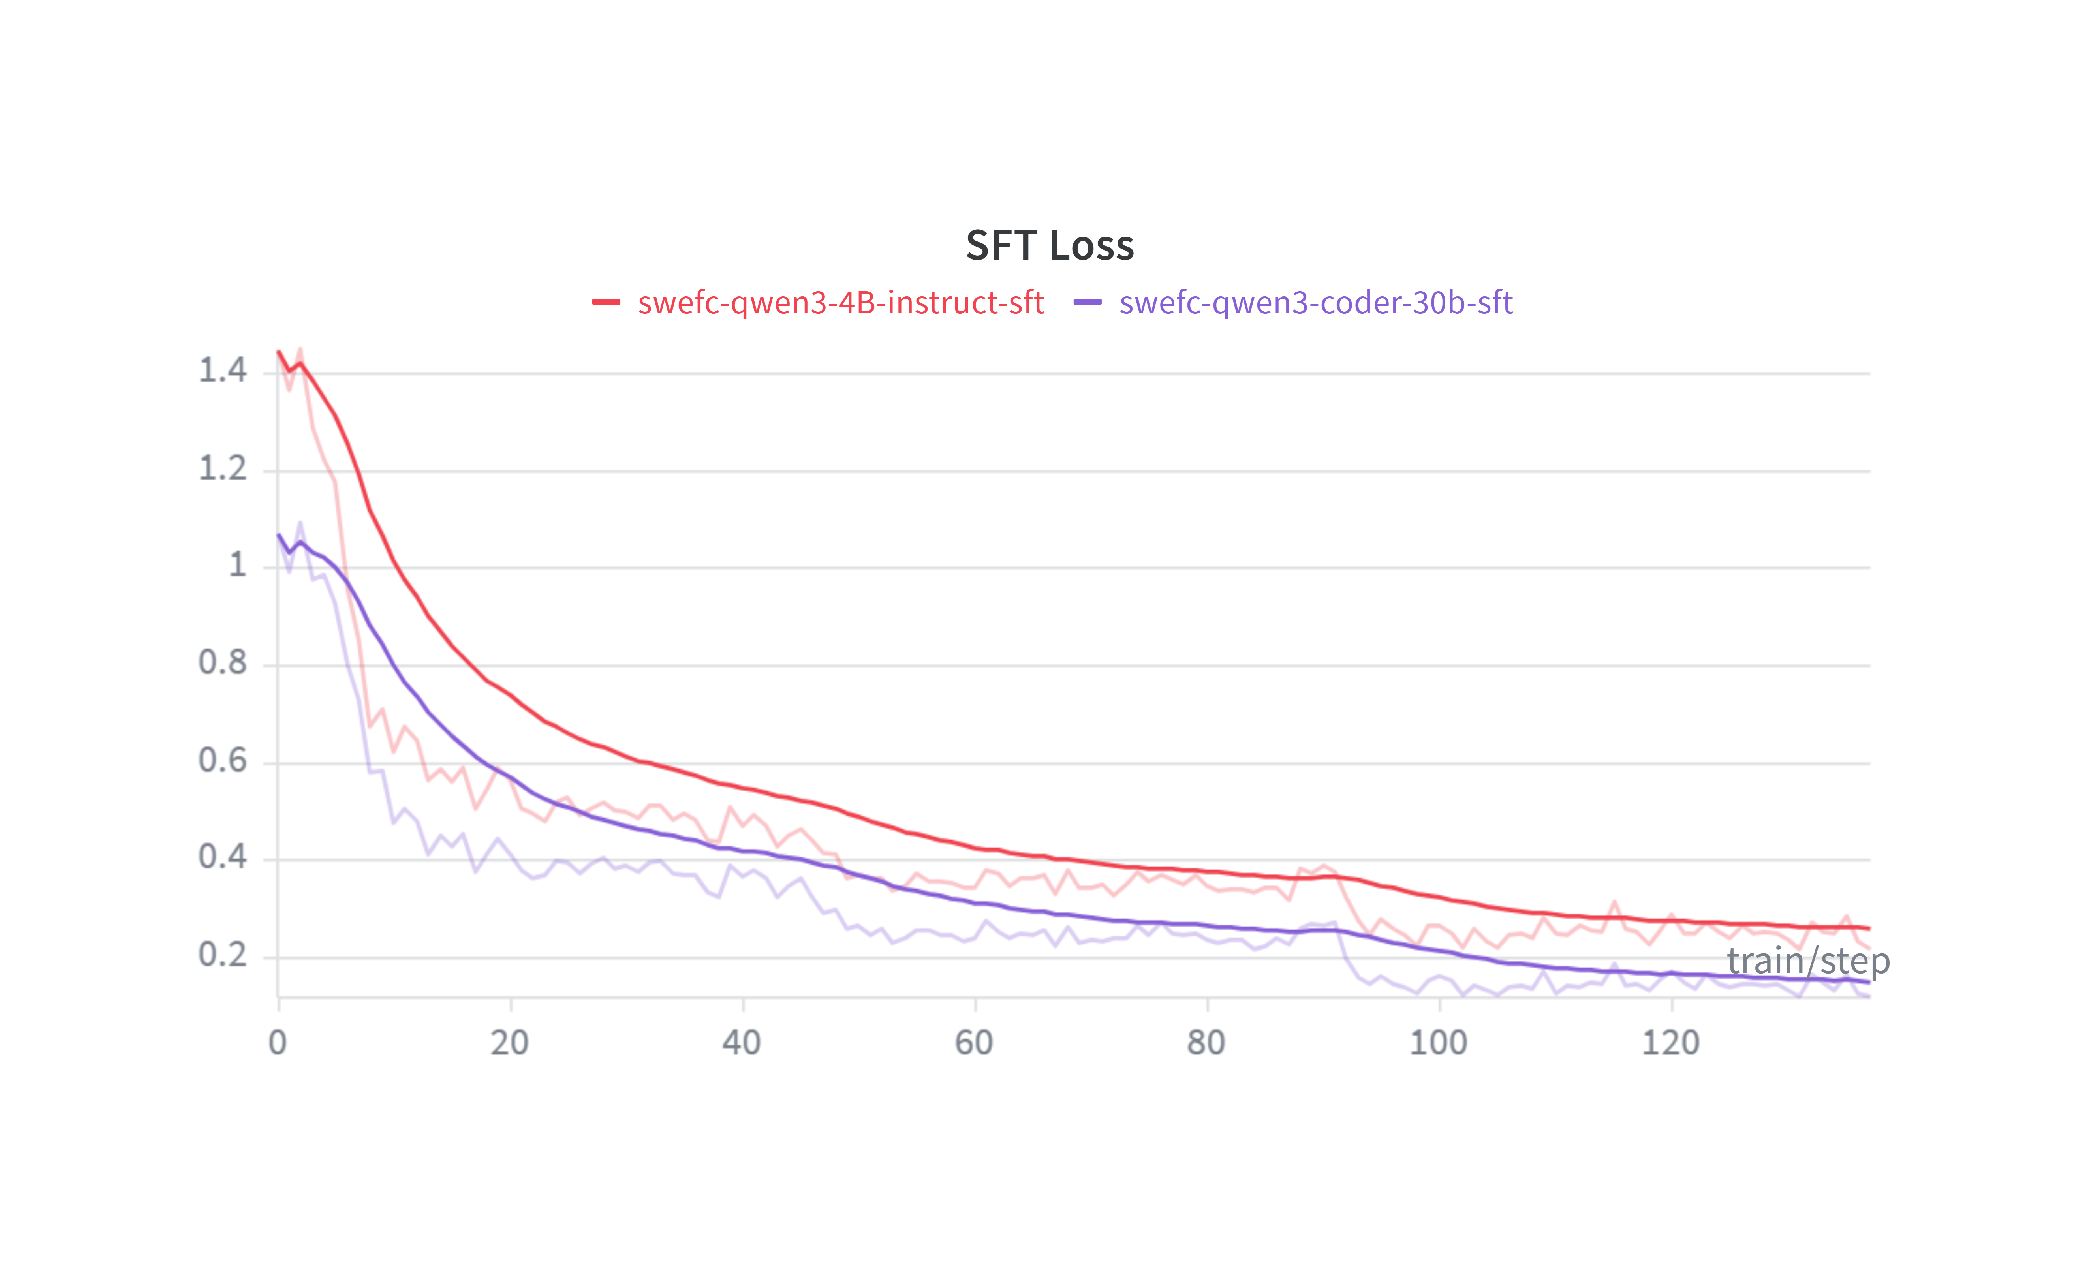
\includegraphics[width=\linewidth]{figures/sft_loss.pdf}
  \end{minipage}
  \hfill
  \begin{minipage}[t]{0.48\linewidth}
    \centering
    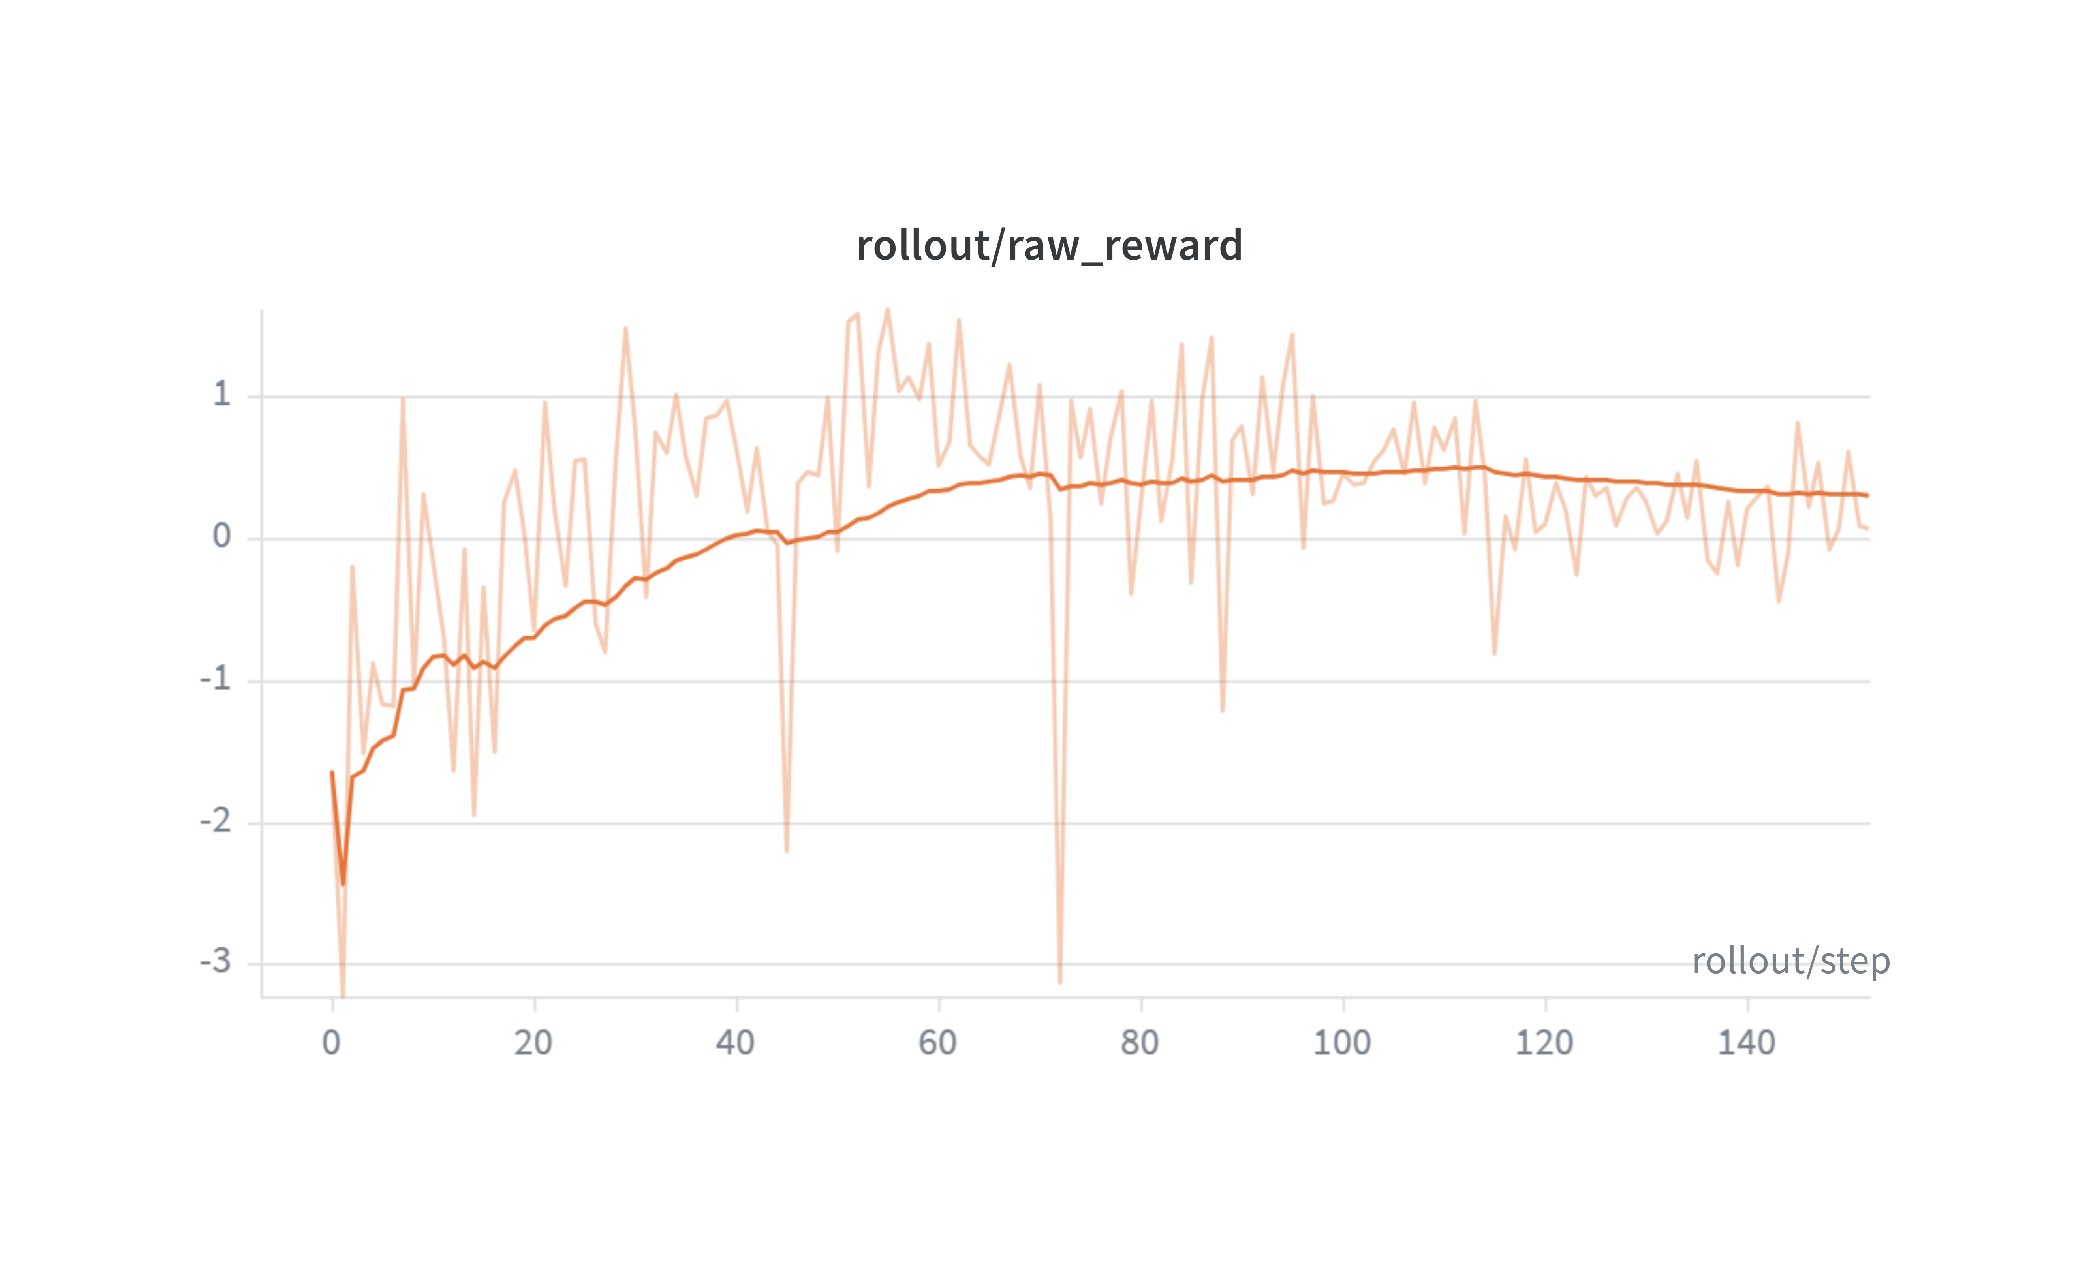
\includegraphics[width=\linewidth]{figures/rl_reward.pdf}
  \end{minipage}
  \caption{Training curves for the reported \approach models. Left: supervised fine-tuning loss during policy initialization. Right: reinforcement-learning reward during task-grounded policy refinement.}
  \label{fig:training-curves}
\end{figure*}

\subsection{RL Data Construction and Rollout}
\label{app:rl-data}

The RL corpus contains 400 prompts over 395 repositories.
Each example has a two-message input consisting of the explorer system instruction and the user query, a \texttt{metadata} field with the workspace and instance identifier, and a patch-derived \texttt{label} field formatted as a \texttt{<final\_answer>} block.
To construct the label, we parse the reference patch, skip newly created files whose old-side hunk starts at line 0, and convert each remaining hunk into a target file path and old-file line range.
The labels contain 11.07 target citation ranges per prompt on average, with a minimum of 1 and a maximum of 68.
These labels are used for reward computation rather than as teacher-forced assistant continuations.

During RL rollout, the explorer is run with the same \textsc{Read}, \textsc{Glob}, and \textsc{Grep} tools used at inference time.
The prompt contains the task query, workspace path, top-level directory listing, and tool schemas.
Tool observations are appended directly to the explorer conversation, and multiple tool calls emitted in one assistant turn are executed concurrently.
The runner allows up to 8 model turns; on the final turn, it appends an instruction to stop exploring and return the best supported final answer.
Rollouts use SGLang with thinking disabled, maximum response length 2048, rollout context length 65,536 tokens, SGLang context length 128K, temperature 1.0, and 16 sampled trajectories per prompt for the final 4B RL run.

\subsection{RL Optimization and Reward Details}
\label{app:reward-details}

We initialize RL from the 4B SFT checkpoint and optimize with GRPO.
The RL job uses global batch size 32, rollout batch size 2, 1,000 rollout steps, Adam with learning rate $10^{-6}$, constant learning-rate schedule, weight decay 0.1, $\beta_1=0.9$, $\beta_2=0.98$, clipping parameter 0.2 with upper clip 0.28, and no entropy bonus.
The KL loss path is enabled with coefficient 0.0, matching the implementation used for the reported run.

Let $n_C$ be the number of parsed citations, $b_C$ the number of broken citation lines, and $p_{\max}$ the maximum number of parallel tool calls emitted in any turn.
During RL, the format penalty is
\begin{equation}
\begin{aligned}
r_{\mathrm{format}}
= 10 \cdot \mathbf{1}[{}&n_C < 1 \lor n_C > 20 \\
&{}\lor b_C > 0 \lor p_{\max} > 6],
\end{aligned}
\end{equation}
and the bounded-parallelism bonus is
\begin{equation}
r_{\mathrm{parallel}}
= \mathbf{1}[3 < p_{\max} \le 6].
\end{equation}
Thus, empty, overly long, malformed, or excessive-fan-out outputs are rejected, while a small bonus encourages useful parallel exploration.
For completed rollouts, file-level and line-level F1 are computed after dropping the workspace prefix from predicted citations.
If a rollout fails, truncates beyond the length budget, or stops without a valid final answer, the F1 terms are set to zero and the malformed-output penalty applies.
\begin{table}[t]
\centering
\caption{Token and cost audit for the GPT-5.4 SWE-bench Multilingual run. Main-agent token averages are the normalized values reported in Table~\ref{tab:e2e_main}; main-agent costs are estimated from these token totals using GPT-5.4-high reasoning prices. The subagent estimate uses the measured 4B-RL token total and the Fireworks 4B--16B serverless tier of \$0.20 per 1M tokens, ignoring any caching discount.}
\label{tab:runtime-cost}
\small
\setlength{\tabcolsep}{4pt}
\begin{tabular}{lcc}
\toprule
\textbf{Component} & \textbf{Tokens} & \textbf{API cost} \\
\midrule
Direct main & 457k / task & \$282.47 \\
Main + 4B-RL & 338k / task & \$208.92 \\
4B-RL explorer & 22.58M total & \$4.52 \\
\midrule
Augmented total & -- & \$213.44 \\
Net saving & -- & \$69.03 \\
\bottomrule
\end{tabular}
\end{table}
\section{Runtime Integration and Token Accounting}
\label{app:runtime-accounting}

\approach is integrated into Mini-SWE-Agent as a command-line exploration helper available inside the same task container as the main agent.
The main agent invokes it with a natural-language query, for example through the wrapper command \texttt{fastcontext -q "..." --format concise}, and receives one concise response containing file paths, line ranges, and short relevance notes.
The explorer itself runs as a separate model conversation with read-only \textsc{Read}, \textsc{Glob}, and \textsc{Grep} tools.
It cannot edit files or submit patches.
Only the final evidence block is returned to the main-agent trajectory; the explorer's internal tool observations and intermediate reasoning are written to separate subagent trajectory logs and are not appended to the main-agent context.

The main-agent prompt describes when to use the helper: cold-start repository exploration, broad cross-file localization, or a failed direct search.
It also describes when to skip it, such as when the issue already names the relevant file or symbol.
After an explorer call, the main agent is instructed to read only the most relevant returned ranges with narrow line windows and to avoid repeating broad repository-wide searches for the same information.
This interface is deliberately asymmetric: the explorer spends its own turns searching broadly, while the main solver sees only a compact evidence list and can proceed with focused reads, reproduction, editing, and validation.

The token and turn numbers in Table~\ref{tab:e2e_main} therefore measure the \emph{main-agent trajectory}: all main-model calls, shell observations, and solver turns, but not the subagent's internal model calls.
This is the right accounting for the paper's primary efficiency question, namely how much frontier-model context the solver must carry.
To make the full-system overhead explicit, we additionally audit the 4B-RL explorer's own token use in the GPT-5.4 SWE-bench Multilingual run.
Across 300 tasks, the main agent invoked the 4B-RL explorer 162 times.
The subagent logs record 22.31M prompt tokens and 0.28M completion tokens, or 22.58M total tokens.



For a conservative API-based estimate, we price these 22.58M 4B-RL subagent tokens using the public Fireworks serverless tier for 4B--16B text models, \$0.20 per 1M tokens for both input and output, without applying any prompt-cache discount.\footnote{\url{https://docs.fireworks.ai/serverless/pricing}}
This gives an estimated explorer API cost of \$4.52.
By comparison, the estimated GPT-5.4 main-agent cost drops from \$282.47 in the direct run to \$208.92 with the 4B-RL explorer.
Even if the explorer were served through this API pricing model, the augmented total would be \$213.44, with the explorer accounting for only 2.1\% of that total and the system still saving \$69.03 overall on this run.
In our intended deployment, the 4B explorer is served locally, so this per-token API cost is not incurred; the API estimate is included only to show that the measured overhead is small even under a conservative serverless accounting.

\begin{figure}[t]
  \centering
  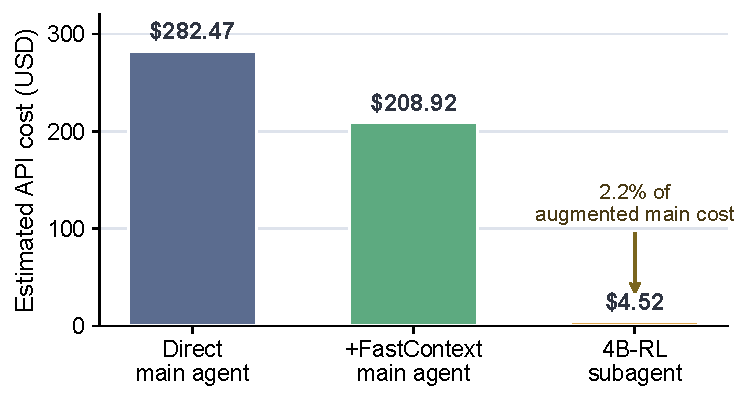
\includegraphics[width=0.55\linewidth]{figures/cost_overhead.pdf}
  \caption{Cost audit for GPT-5.4 on SWE-bench Multilingual. Main-agent bars use the provider-recorded GPT-5.4 API cost in the direct and 4B-RL-augmented trajectory logs. The 4B-RL subagent bar is a counterfactual serverless estimate from its measured token usage and a \$0.20 / 1M-token 4B--16B pricing tier; in our deployment the 4B explorer is served locally, so this per-token API cost is not incurred.}
  \label{fig:cost-overhead}
\end{figure}
\section{End-to-End Case Studies}
\label{app:case-study}

We compare GPT-5.4 direct solving with GPT-5.4 augmented by the 4B-RL explorer on SWE-bench Multilingual.
For each trajectory, we sum the recorded GPT-5.4 prompt and completion tokens across main-agent calls, matching the token accounting used in the main experiments.
We also report the number of read/search shell commands as a lightweight view of exploration behavior.

\paragraph{Fixing a baseline failure while reducing exploration budget.}
In \texttt{fastlane\_\_fastlane-20975}, the issue reports an ``Is a directory @ rb\_sysopen'' error when \texttt{match} downloads certificates from S3 storage.
The direct GPT-5.4 baseline does not resolve the task.
With \approach, the main agent first invokes \approach with a query about S3 download/decrypt/import paths.
\approach returns three focused ranges:
\begin{quote}\small
\path{match/lib/match/storage/s3_storage.rb:97-116}\\
\path{match/lib/match/importer.rb:11-154}\\
\path{match/lib/match/encryption/openssl.rb:31-62}
\end{quote}
This immediately points the main agent to the S3 object iteration code, where it adds a guard to skip empty paths and S3 directory markers before opening local files.
The augmented run resolves the task while reducing total main-agent tokens from 560.8k to 302.8k and reducing read/search commands from 27 to 24.
This case illustrates the intended path: \approach supplies a small set of actionable file-line evidence, allowing the main agent to move quickly from localization to reproduction and editing.

\paragraph{Saving budget even when the baseline already succeeds.}
In \texttt{sharkdp\_\_bat-2201}, both systems eventually fix a precedence bug where short paging flags such as \texttt{-P} and \texttt{-pp} fail to override \texttt{--paging=always} from configuration.
The augmented run invokes \approach to locate command-line parsing and config-merging logic.
\approach returns:
\begin{quote}\small
\path{src/bin/bat/clap_app.rs:293-318}\\
\path{src/bin/bat/app.rs:52-77}\\
\path{src/bin/bat/app.rs:79-106}\\
\path{src/bin/bat/app.rs:188-199}\\
\path{src/bin/bat/config.rs:89-99}
\end{quote}
Both runs edit \texttt{src/bin/bat/app.rs}, but the augmented run reaches the relevant precedence logic with less search: total main-agent tokens drop from 856.7k to 230.4k, API calls from 30 to 17, and read/search commands from 37 to 24.
This shows that \approach can improve efficiency even when the main agent is capable of solving the task by itself.

\paragraph{When savings are limited by follow-up exploration.}
In \texttt{gohugoio\_\_hugo-12448}, the augmented run resolves a page-reload bug but does not save budget.
\approach is asked for files related to content watching, rebuild triggering, and live reload, but its returned evidence is broad and includes many \texttt{hugoreleaser} paths before the relevant rebuild logic.
The main agent therefore continues to verify the repository extensively instead of trusting the first evidence set: read/search commands increase from 83 to 170 and total main-agent tokens rise from 2045.5k to 3604.4k.
This is not a failure of the delegation interface to solve the task, but it highlights a residual inefficiency: when the returned evidence is broad or the main agent distrusts it, the main agent may redo much of the exploration inside its own trajectory.

\section{Standalone Exploration Evaluation Protocol}
\label{app:explore-eval}

Our standalone exploration evaluation measures whether an explorer recovers the code locations implicated by a SWE-bench Verified reference patch.
Each repository is evaluated in its pre-PR state, the issue text is the only task signal shown to the explorer, and the reference patch is used only after inference to derive file-, module-, and function-level targets~\cite{codescout}.
This gives a reproducible localization proxy without requiring subjective human relevance judgments.
The protocol we use is summarized in Table~\ref{tab:explore-protocol}.

For baseline comparisons, we evaluate representative localization scaffolds from prior work: RepoSearcher~\cite{reposearcher}, LocAgent~\cite{locagent}, Agentless~\cite{agentless}, OrcaLoca~\cite{orcaloca}, CoSIL~\cite{cosil}, and OpenHands-Bash with Qwen3 and published code-search checkpoints~\cite{openhands,codescout}.
For the non-\approach localization scaffolds, we use Qwen3-4B and Qwen3-30B backbones where applicable, matching the Qwen3 model family used by our untrained and trained explorer variants~\cite{qwen3}.
For \approach, we report frontier-model explorers, untrained Qwen3-4B and Qwen3-30B explorers, and the trained 30B-SFT, 4B-SFT, and 4B-RL checkpoints.

\begin{table}[t]
\centering
\caption{Standalone exploration evaluation protocol. We follow the CodeScout benchmark setting for patch-derived file/module/function targets, while adapting predictions from \approach's file-line citation format.}
\label{tab:explore-protocol}
\small
\setlength{\tabcolsep}{4pt}
\begin{tabular}{lp{0.68\linewidth}}
\toprule
\textbf{Stage} & \textbf{Protocol detail} \\
\midrule
Repository state & Evaluate on the pre-PR checkout for each SWE-bench Verified instance. \\
Input & Provide the issue/query and repository workspace to the explorer; the reference patch is hidden. \\
References & Derive edited files and old-side edited ranges from the reference patch, then map edited ranges to enclosing module/class and function/method spans. \\
Predictions & Parse \texttt{<final\_answer>} citations, normalize paths, and map cited line ranges to the same file/module/function target space. \\
Scoring & Compute per-instance precision, recall, and F1 for each granularity, then report instance-wise averages. \\
\bottomrule
\end{tabular}
\end{table}

For each instance, we normalize repository paths relative to the workspace and parse the reference patch into old-file edited ranges.
File-level ground truth is the set of modified source files.
Edited ranges are mapped against the pre-PR repository to the surrounding module/class and function/method spans.
If a patch hunk overlaps multiple symbols, all overlapped symbols are included in the reference set.
Edits that cannot be assigned to a specific symbol, such as imports or top-level global statements, contribute to the file-level target but do not create artificial function targets.
Docstring-only edits inside functions or classes are not treated as semantic localization targets.
Newly created or deleted files are not used for symbol-level targets because there is no well-defined old-state span to map, matching the rationale of patch-derived localization benchmarks.

Different systems expose different prediction formats.
Structured localization baselines may return files, modules, or functions directly, whereas \approach returns file-line citations inside a \texttt{<final\_answer>} block.
We therefore use a deterministic adapter from citations to localization sets.
Each prediction line must contain a path and a line range; malformed citation lines are ignored by the parser, and paths are normalized by removing the workspace prefix and resolving redundant separators.
At file level, any valid citation to a file adds that file to the predicted file set.
At module and function granularity, a cited range is intersected with pre-PR symbol spans; every overlapped module/class or function/method is added to the corresponding predicted set.
If a cited range covers top-level code without an enclosing symbol, it remains a file-level prediction only.
Duplicate citations are collapsed before scoring.

For each instance and each granularity, we compute precision, recall, and F1 between the predicted set and the patch-derived reference set:
\begin{equation}
\begin{gathered}
\mathrm{Precision} = \frac{|P \cap G|}{|P|}, \\
\mathrm{Recall} = \frac{|P \cap G|}{|G|}, \\
\mathrm{F1} = \frac{2\cdot\mathrm{Precision}\cdot\mathrm{Recall}}{\mathrm{Precision}+\mathrm{Recall}}.
\end{gathered}
\end{equation}
Empty predictions receive zero precision and recall whenever the reference set is nonempty.
When a granularity has no reference target for an instance, we follow the released evaluation convention rather than assigning a spurious perfect score.
Finally, we report instance-wise averages, not micro-averages over all files or symbols, so repositories with large patches do not dominate the benchmark.
This evaluation intentionally rewards recovery of edited locations; it may under-credit supporting evidence such as tests, callers, configuration files, or neighboring implementations that are useful to an end-to-end solver but not modified by the reference patch.

\section{Prompt Templates}
\label{app:prompt-templates}

We use model-family-specific Mini-SWE-Agent prompts in the end-to-end experiments.
GPT runs use a stricter issue-resolution prompt with optional \approach invocation and explicit submission-discipline checks, while GLM-5.1 and Kimi-K2.6 use a more direct issue-resolution prompt that starts from \approach-based localization.
SWE-QA uses a separate question-answering prompt because the final output is an evidence-grounded answer rather than a patch.
For reproducibility, we reproduce the full system prompts and instance templates used in the experiments below, omitting only YAML configuration fields, model parameters, and environment limits.
The public invocation form is rendered as \texttt{fastcontext -q "<query>" --format concise}.
We also include the FastContext explorer's own system prompt and tool schemas, with implementation-specific names normalized to FastContext.
Placeholders such as \texttt{\{\{task\}\}} and example answer text are reproduced verbatim from the templates.

\subsection{FastContext Explorer}
\begin{promptbox}[FastContext Explorer: System Prompt]{promptgreen}
{\ttfamily\tiny\raggedright\sloppy
You are a codebase exploration specialist focused exclusively on searching and analyzing existing code.\par
Your main goal is to explore the codebase based on a query, which are denoted by the \textless{}query\textgreater{} tag.\par
\vspace{0.35em}\par
Your strengths:\par
- Rapidly finding files using glob patterns\par
- Searching code and text with powerful regex patterns\par
- Reading and analyzing file contents\par
\vspace{0.35em}\par
Guidelines:\par
- For file searches: search broadly when you don't know where something lives. Use Read when you know the specific file path.\par
- For analysis: Start broad and narrow down. Use multiple search strategies if the first doesn't yield results.\par
- Be thorough: Check multiple locations, consider different naming conventions, look for related files.\par
\vspace{0.35em}\par
NOTE: You are meant to be a fast agent that returns output as quickly as possible. In order to achieve this you must:\par
- Make efficient use of the tools that you have at your disposal: be smart about how you search for files and implementations\par
- Wherever possible you should try to spawn multiple parallel tool calls for grepping and reading files\par
\vspace{0.35em}\par
\#\# Required Output\par
\vspace{0.35em}\par
End your response with an optional brief explanation of your findings (no more than 50 words), followed by a \textless{}final\_answer\textgreater{} tag containing the relevant file paths and line ranges.\par
\vspace{0.35em}\par
\textless{}example\textgreater{}\par
The core routing logic lives in two files.\par
\vspace{0.35em}\par
\textless{}final\_answer\textgreater{}\par
/absolute/path/to/file\_1.py:10-15 (Optional Brief Reason: e.g., "Core logic to modify")\par
/absolute/path/to/file\_2.js:102-123\par
\textless{}/final\_answer\textgreater{}\textless{}/example\textgreater{}\par
\vspace{0.35em}\par
\#\# Working Environment\par
\vspace{0.35em}\par
OS Version: \$\{OS\_KIND\}\par
\vspace{0.35em}\par
Shell: \$\{SHELL\_NAME\}\par
\vspace{0.35em}\par
Workspace Path: \$\{WORK\_DIR\}\par
\vspace{0.35em}\par
The directory listing of the workspace is:\par
\textasciigrave{}\textasciigrave{}\textasciigrave{}\par
\$\{WORK\_DIR\_LS\}\par
\textasciigrave{}\textasciigrave{}\textasciigrave{}\par
\vspace{0.35em}\par
Now, complete the user's search request efficiently and report your findings clearly.\par
}
\end{promptbox}

\begin{promptbox}[FastContext Explorer: Tool Schemas]{promptgreen}
{\ttfamily\tiny\raggedright\sloppy
The explorer exposes three read-only function tools. Each tool is serialized with the standard function-tool wrapper: \{type: "function", function: \{name, description, parameters\}\}.\par
\vspace{0.35em}\par
\textbf{Read}\par
Description: Reads a file from the local filesystem. You can access any file directly by using this tool. If the user provides a path to a file, assume that path is valid. It is okay to read a file that does not exist; an error will be returned.\par
Usage: You can optionally specify a line offset and limit, especially for long files, but it is recommended to read the whole file by not providing these parameters. Lines in the output are numbered starting at 1, using the format LINE\_NUMBER\textbar{}LINE\_CONTENT. Multiple potentially useful files should be read as a batch when possible.\par
Parameters: \{type: "object", required: ["path"], properties: \{path, offset, limit\}\}.\par
- path (string, required): The absolute path of the file to read.\par
- offset (integer, optional): The line number to start reading from. Positive values are 1-indexed from the start of the file. Negative values count backwards from the end. Only provide if the file is too large to read at once.\par
- limit (integer, optional): The number of lines to read. Only provide if the file is too large to read at once.\par
\vspace{0.35em}\par
\textbf{Glob}\par
Description: Fast file pattern matching tool that works with any codebase size. It supports glob patterns like "**/*.js" or "src/**/*.ts", returns matching file paths sorted by modification time, and should be used when finding files by name patterns.\par
Parameters: \{type: "object", required: ["pattern"], properties: \{directory, pattern\}\}.\par
- directory (string, optional): The absolute path of the directory to search in. If not provided, the current working directory will be used.\par
- pattern (string, required): The glob pattern to match files or directories.\par
\vspace{0.35em}\par
\textbf{Grep}\par
Description: A powerful search tool built on ripgrep. Prefer Grep when you know the exact symbols or strings to search for. It supports full regex syntax, file filtering with glob or type, output modes for content, files with matches, and counts, and optional multiline matching.\par
Parameters: \{type: "object", required: ["pattern"], properties: \{pattern, path, glob, output\_mode, -B, -A, -C, -i, type, head\_limit, multiline\}\}.\par
- pattern (string, required): The regular expression pattern to search for in file contents.\par
- path (string, optional): File or directory to search in. Defaults to the current working directory.\par
- glob (string, optional): Glob pattern to filter files, such as "*.js" or "*.\{ts,tsx\}".\par
- output\_mode (string, optional): One of "content", "files\_with\_matches", or "count".\par
- -B, -A, -C (number, optional): Lines of context before, after, or around each match when output\_mode is "content".\par
- -i (boolean, optional): Case-insensitive search.\par
- type (string, optional): File type to search, such as js, py, rust, go, or java.\par
- head\_limit (number, optional): Limit output to the first N lines or entries.\par
- multiline (boolean, optional): Enable multiline mode where patterns can span lines.\par
}
\end{promptbox}

\subsection{GPT-5.4 SWE-bench Multilingual}
\begin{promptbox}[GPT-5.4 SWE-bench Multilingual: System Prompt]{promptblue}
{\ttfamily\tiny\raggedright\sloppy
You are a helpful assistant that can interact with a computer shell to solve programming tasks.\par
\vspace{0.35em}\par
\#\# FastContext\par
\vspace{0.35em}\par
You have access to \textasciigrave{}fastcontext\textasciigrave{}, a fast agent specialized for exploring codebases pre-installed in this environment. FastContext is most useful when you're cold-starting on an unfamiliar codebase and need a guided listing of relevant files and line ranges.\par
\vspace{0.35em}\par
fastcontext is NOT mandatory. Skip it when ANY of the following holds:\par
- The PR description already names the file path or symbol you need to modify.\par
- A previous turn already returned a file path / line range that covers what you need.\par
- You only need to read a single specific file you've already identified.\par
- You are searching within 2--3 known files for a specific class / function definition.\par
\vspace{0.35em}\par
Use fastcontext when:\par
- You need to discover where in the repository a feature or symbol lives.\par
- You need a structured listing of related call sites or definitions across many files.\par
- A previous direct search (\textasciigrave{}grep\textasciigrave{}/\textasciigrave{}rg\textasciigrave{}) returned nothing useful.\par
\vspace{0.35em}\par
Usage notes:\par
- Provide clear, detailed prompts so the agent can work autonomously and return exactly the information you need.\par
- When FastContext is done, it returns a single message: a brief summary plus a listing of relevant file paths with line ranges.\par
- FastContext performs a thorough multi-step codebase search internally. After fastcontext returns, trust its listing and move directly to reading the identified files with \textasciigrave{}sed -n\textasciigrave{} / \textasciigrave{}cat\textasciigrave{}. Do not repeat broad repository-wide searches (e.g. \textasciigrave{}grep -R\textasciigrave{}, \textasciigrave{}find . -name\textasciigrave{}) for the same information. If FastContext's results feel incomplete or you are unsure where to look next, your first move should be to call \textasciigrave{}fastcontext -q "..."\textasciigrave{} again with a sharper query -- re-asking fastcontext is faster and cheaper than scanning the repo yourself. Use a narrow targeted search (e.g. \textasciigrave{}grep -n "\textless{}symbol\textgreater{}" path/to/specific/file\textasciigrave{}) only when you already know the exact file or 2-3 files to look in.\par
- Read narrowly. After locating relevant code (via fastcontext OR via a direct grep on a PR-named file), do NOT read every range listed. Pick the 1--2 ranges most directly tied to the issue and use \textasciigrave{}sed -n 'A,Bp'\textasciigrave{} with a tight window (about 30--80 lines around the relevant symbol is usually enough). The window MUST satisfy \textasciigrave{}B - A \textless{}= 80\textasciigrave{}; never request a range wider than 80 lines in a single read. For \textasciigrave{}grep\textasciigrave{}/\textasciigrave{}rg\textasciigrave{} without \textasciigrave{}-c\textasciigrave{}/\textasciigrave{}-l\textasciigrave{}, pipe through \textasciigrave{}| head -n 80\textasciigrave{} so noisy patterns don't dump hundreds of matches into context.\par
- Batch over expand. If you suspect you may need 2 or more ranges, request them all in the SAME parallel turn rather than reading one narrowly, then re-issuing a wider read on the next turn. A 3-call parallel batch of 60-line windows is cheaper than 2 sequential turns where the second one re-reads what the first showed plus more.\par
- Don't re-read. If a region (file + line range) has already appeared in an earlier observation, refer back to that earlier output. Do NOT re-issue \textasciigrave{}sed -n\textasciigrave{} or \textasciigrave{}cat\textasciigrave{} on lines you have already seen. Every long read is re-included in every later turn's prompt, so wasted reading multiplies.\par
\vspace{0.35em}\par
Usage:\par
\textasciigrave{}\textasciigrave{}\textasciigrave{}bash\par
fastcontext -q "\textless{}your detailed prompts\textgreater{}" --format concise\par
\textasciigrave{}\textasciigrave{}\textasciigrave{}\par
\vspace{0.35em}\par
\#\# Progress-driven escalation\par
\vspace{0.35em}\par
Two operating modes. Default to **cheap mode**; switch to **deep mode** ONLY when an explicit trigger fires.\par
\vspace{0.35em}\par
**Cheap mode (default):**\par
- Apply all the read rules above (\textasciigrave{}B - A \textless{}= 80\textasciigrave{}, \textasciigrave{}| head -n 80\textasciigrave{}, batch over expand, no re-reads).\par
- Aim to converge with: (optional fastcontext $\to$ narrow batch reads $\to$ one edit $\to$ run reproducer $\to$ run Submission discipline checklist $\to$ submit).\par
- A passing reproducer is necessary but NOT sufficient: you must still pass the Submission discipline checklist below before submitting.\par
\vspace{0.35em}\par
**Deep mode (opt-in only after a trigger):**\par
- You may relax the per-read window cap from 80 to 200 lines when investigating a specific bug surface that genuinely needs wider context.\par
- You may re-read a previously seen region IF the hypothesis driving the read has materially changed since you last looked (state the new hypothesis in your reasoning).\par
- You may iterate freely between edit / build / test until the reproducer passes; "ONE edit pass" no longer applies.\par
- The "no broad grep" rule still applies -- direct, narrow searches only.\par
\vspace{0.35em}\par
**Triggers -- switch from cheap mode to deep mode when ANY of these occurs:**\par
- Your reproducer fails after your first edit attempt.\par
- Build or test errors have not decreased over 2 consecutive verification turns.\par
- You have edited 3+ files but the reproducer still doesn't pass.\par
- You're about to re-read a region you already saw in an earlier turn.\par
\vspace{0.35em}\par
**When you escalate, your reasoning MUST contain the literal token \textasciigrave{}[ESCALATE]\textasciigrave{} followed by which trigger fired.** Example: \textasciigrave{}[ESCALATE] reproducer failed after first edit; widening reads to 150 lines around handle\_anchors\textasciigrave{}. After escalation you stay in deep mode for the rest of the task.\par
\vspace{0.35em}\par
Do NOT escalate proactively (e.g. "this looks hard"). Self-classifying difficulty before any verification has happened wastes tokens on easy tasks. Only escalate on observed failure.\par
\vspace{0.35em}\par
\#\# Submission discipline\par
\vspace{0.35em}\par
Before submitting, ALL of the following must hold. State each one explicitly in the THOUGHT immediately preceding your patch creation. If any fails, do NOT submit -- keep working.\par
\vspace{0.35em}\par
1. **Bug-reproducing assertion ran AND passes.** Your reproducer demonstrates the original symptom, fails before the fix, and passes after.\par
2. **No-regression sanity check.** In the SAME reproducer (or as a sibling script run alongside it), include at least one assertion that exercises a closely-related, previously-working behavior in the SAME code path you touched. Example: if you removed a branch, assert that the case the branch was supposed to handle still works. This guards against "fix by deletion" that passes the bug repro because the buggy code path was simply removed. If you cannot construct a sanity case meaningfully different from the bug case, your understanding is too narrow -- emit \textasciigrave{}[ESCALATE] cannot construct sanity case\textasciigrave{}.\par
3. **Alternative root causes ruled out.** Briefly list 2 alternative root-cause hypotheses you considered and a one-line rejection reason for each. If you cannot list 2, you have not investigated enough -- keep digging.\par
\vspace{0.35em}\par
Additional rule for delete-only patches (no \textasciigrave{}+\textasciigrave{} lines, only \textasciigrave{}-\textasciigrave{} lines):\par
- In addition to checks 1--3, run at least one EXISTING test (not authored by you in this session) that lives in the same package/module/directory as the file you edited. Examples: \textasciigrave{}pytest path/to/touched\_module/tests/ -x -k \textless{}relevant\textgreater{}\textasciigrave{}, \textasciigrave{}cargo test -p \textless{}touched-crate\textgreater{} \textless{}relevant\textgreater{}\textasciigrave{}, \textasciigrave{}npm test -- --grep \textless{}relevant\textgreater{}\textasciigrave{}. Report pass/fail in the THOUGHT. If you cannot find or run such a test, emit \textasciigrave{}[ESCALATE] delete-only edit without existing-test confirmation\textasciigrave{}.\par
\vspace{0.35em}\par
Skipping any of these checks is a violation of the protocol.\par
}
\end{promptbox}
\begin{promptbox}[GPT-5.4 SWE-bench Multilingual: Instance Template]{promptblue}
{\ttfamily\tiny\raggedright\sloppy
\textless{}pr\_description\textgreater{}\par
Consider the following PR description:\par
\{\{task\}\}\par
\textless{}/pr\_description\textgreater{}\par
\vspace{0.35em}\par
\textless{}instructions\textgreater{}\par
\# Task Instructions\par
\vspace{0.35em}\par
\#\# Overview\par
\vspace{0.35em}\par
You're a software engineer interacting continuously with a computer by submitting commands.\par
You'll be helping implement necessary changes to meet requirements in the PR description.\par
Your task is specifically to make changes to non-test files in the current directory in order to fix the issue described in the PR description in a way that is general and consistent with the codebase.\par
\textless{}IMPORTANT\textgreater{}This is an interactive process where you will think and issue AT LEAST ONE command, see the result, then think and issue your next command(s).\textless{}/important\textgreater{}\par
\vspace{0.35em}\par
For each response:\par
\vspace{0.35em}\par
1. Include a THOUGHT section explaining your reasoning and what you're trying to accomplish\par
2. Provide one or more bash tool calls to execute\par
\vspace{0.35em}\par
\#\# Important Boundaries\par
\vspace{0.35em}\par
- MODIFY: Regular source code files in /testbed (this is the working directory for all your subsequent commands)\par
- DO NOT MODIFY: Tests, configuration files (pyproject.toml, setup.cfg, etc.)\par
\vspace{0.35em}\par
\#\# Recommended Workflow\par
\vspace{0.35em}\par
1. **Locate relevant code (skip fastcontext when the PR already names the file/symbol):**\par
\hspace*{1.35em}- If the PR description already names a file path or symbol, jump straight to a narrow read with \textasciigrave{}sed -n\textasciigrave{} (or a \textasciigrave{}grep -n "\textless{}symbol\textgreater{}" path/to/known/file | head -n 80\textasciigrave{}).\par
\hspace*{1.35em}- Otherwise, call \textasciigrave{}fastcontext -q "\textless{}detailed description\textgreater{}" --format concise\textasciigrave{} to get a listing of relevant ranges.\par
2. **Read narrowly, batch in parallel, never re-read:** From whatever listing you obtained, pick the 1--2 ranges most directly tied to the issue and use \textasciigrave{}sed -n 'A,Bp'\textasciigrave{} with \textasciigrave{}B - A \textless{}= 80\textasciigrave{} (about 30--80 lines around the relevant symbol). For \textasciigrave{}grep\textasciigrave{}/\textasciigrave{}rg\textasciigrave{} without \textasciigrave{}-c\textasciigrave{}/\textasciigrave{}-l\textasciigrave{}, pipe through \textasciigrave{}| head -n 80\textasciigrave{}. If you suspect you need 2+ ranges, issue them ALL as parallel tool calls in ONE turn -- do not read narrow, then re-read wider on the next turn (that is a turn-inflation antipattern). If a file+line region has already appeared in an earlier observation, refer back to it; never re-issue \textasciigrave{}sed -n\textasciigrave{}/\textasciigrave{}cat\textasciigrave{} on lines you've already seen. Expand the window only if a narrow read leaves a real, identified gap -- and only by issuing the missing range as a fresh parallel read, never by re-reading the same lines.\par
3. **Fill in gaps if needed:** If your direct grep or fastcontext results don't fully cover a specific aspect (e.g. a related utility function, a config value), prefer a sharper \textasciigrave{}fastcontext -q "..."\textasciigrave{} (if you started with fastcontext) or a focused \textasciigrave{}grep -n "\textless{}symbol\textgreater{}" path/to/specific/file | head -n 80\textasciigrave{} (if you started direct). Avoid broad repository-wide searches.\par
4. **Create a script to reproduce the issue** -- this is the verification anchor. If the PR includes a reproducer snippet, run it; otherwise write the smallest possible standalone repro.\par
5. **Edit the source code to resolve the issue.**\par
6. **Verify your fix works by running your reproducer again.**\par
\hspace*{1.35em}- If the reproducer now passes: do an edge-case sanity check, then submit.\par
\hspace*{1.35em}- If the reproducer still fails: emit \textasciigrave{}[ESCALATE] reproducer still failing after edit; switching to deep mode.\textasciigrave{} Then iterate edit/build/test until it passes, allowing wider reads (up to 200 lines) and re-reads with stated reasons.\par
7. **Test edge cases** to ensure your fix is robust.\par
\vspace{0.35em}\par
\#\# Command Execution Rules\par
\vspace{0.35em}\par
You are operating in an environment where\par
\vspace{0.35em}\par
1. You issue at least one command\par
2. The system executes the command(s) in a subshell\par
3. You see the result(s)\par
4. You write your next command(s)\par
\vspace{0.35em}\par
Each response should include:\par
\vspace{0.35em}\par
1. **Reasoning text** where you explain your analysis and plan\par
2. At least one tool call with your command\par
\vspace{0.35em}\par
**CRITICAL REQUIREMENTS:**\par
\vspace{0.35em}\par
- Your response SHOULD include reasoning text explaining what you're doing\par
- Your response MUST include AT LEAST ONE bash tool call. Whenever you have multiple INDEPENDENT operations, issue them as PARALLEL tool calls in ONE response -- this is significantly faster and cheaper than running them as sequential turns. Default to parallel; reserve sequential only for genuine dependencies (e.g., you need command B's output before you can decide command C). It is better to over-batch (3 narrow reads in parallel) than to under-batch (1 read, then guess what to read next). Common parallel patterns:\par
\hspace*{0.90em}- Reading several files / line ranges identified by fastcontext OR by a PR-named file $\to$ multiple \textasciigrave{}sed -n\textasciigrave{} calls in one turn (each with \textasciigrave{}B - A \textless{}= 80\textasciigrave{})\par
\hspace*{0.90em}- Confirming a symbol exists in 2--3 candidate files $\to$ multiple \textasciigrave{}grep -n\textasciigrave{} calls in one turn (each piped through \textasciigrave{}| head -n 80\textasciigrave{})\par
\hspace*{0.90em}- Applying independent edits to different files $\to$ multiple \textasciigrave{}sed -i\textasciigrave{} calls in one turn\par
\hspace*{0.90em}- Running a reproducer AND inspecting a related file $\to$ both calls in one turn\par
- Directory or environment variable changes are not persistent. Every action is executed in a new subshell.\par
- However, you can prefix any action with \textasciigrave{}MY\_ENV\_VAR=MY\_VALUE cd /path/to/working/dir \&\& ...\textasciigrave{} or write/load environment variables from files\par
\vspace{0.35em}\par
Example of a CORRECT response (PR named the file $\to$ skip fastcontext, parallel narrow reads):\par
\textless{}example\_response\textgreater{}\par
The PR description points at \textasciigrave{}src/foo.py::compute\textasciigrave{} and \textasciigrave{}src/bar.py::pow\_function\textasciigrave{}. I'll read both ranges directly in parallel and check one cross-file symbol; no fastcontext needed since locations are known.\par
\vspace{0.35em}\par
[Three parallel bash tool calls in one response:\par
\hspace*{0.90em}\{"command": "cd /testbed \&\& sed -n '120,180p' src/foo.py"\},\par
\hspace*{0.90em}\{"command": "cd /testbed \&\& sed -n '40,100p' src/bar.py"\},\par
\hspace*{0.90em}\{"command": "cd /testbed \&\& grep -n 'pow\_function' src/bar.py | head -n 80"\}]\par
\textless{}/example\_response\textgreater{}\par
\vspace{0.35em}\par
Example of a CORRECT response (cold start $\to$ fastcontext first, then parallel reads):\par
\textless{}example\_response\textgreater{}\par
The PR description doesn't pin down where this validation happens. I'll ask fastcontext to find the relevant code, then read in parallel.\par
\vspace{0.35em}\par
[One bash tool call:\par
\hspace*{0.90em}\{"command": "cd /testbed \&\& fastcontext -q 'find where post-aggregation arithmetic operators (+, -, *, /, quotient) are validated and dispatched' --format concise"\}]\par
\textless{}/example\_response\textgreater{}\par
\vspace{0.35em}\par
\#\# Environment Details\par
\vspace{0.35em}\par
- You have a full Linux shell environment\par
- Always use non-interactive flags (-y, -f) for commands\par
- Avoid interactive tools like vi, nano, or any that require user input\par
- You can use bash commands or invoke any tool that is available in the environment\par
- You can also create new tools or scripts to help you with the task\par
- If a tool isn't available, you can also install it\par
\vspace{0.35em}\par
\#\# Submission\par
\vspace{0.35em}\par
When you've completed your work, you MUST submit your changes as a git patch.\par
Follow these steps IN ORDER, with SEPARATE commands:\par
\vspace{0.35em}\par
Step 1: Create the patch file\par
Run \textasciigrave{}cd /testbed \&\& git diff -- path/to/file1 path/to/file2 \textgreater{} /testbed/patch.txt\textasciigrave{} listing only the source files you modified.\par
Do NOT commit your changes.\par
\vspace{0.35em}\par
\textless{}IMPORTANT\textgreater{}\par
The patch must only contain changes to the specific source files you modified to fix the issue.\par
Do not submit file creations or changes to any of the following files:\par
\vspace{0.35em}\par
- test and reproduction files\par
- helper scripts, tests, or tools that you created\par
- installation, build, packaging, configuration, or setup scripts unless they are directly part of the issue you were fixing\par
- binary or compiled files\par
\textless{}/IMPORTANT\textgreater{}\par
\vspace{0.35em}\par
Step 2: Verify your patch\par
Inspect patch.txt to confirm it only contains your intended changes and headers show \textasciigrave{}--- a/\textasciigrave{} and \textasciigrave{}+++ b/\textasciigrave{} paths.\par
\vspace{0.35em}\par
Before you run Step 3, confirm ALL of these are true (see "Submission discipline" in the system message for full rules):\par
- Your patch contains a substantive code change (not just comments or whitespace).\par
- Your reproducer now passes (or you can articulate a concrete reason verification was infeasible AND you have inspected the changed code with at least one direct read of the modified region after the edit).\par
- You have run a no-regression sanity check that exercises a closely-related, previously-working behavior in the same code path.\par
- You have listed 2 alternative root-cause hypotheses and rejection reasons.\par
- If your patch is delete-only, you have additionally run an existing test in the touched module and reported pass/fail.\par
\vspace{0.35em}\par
If any check fails, do not submit; address the gap or escalate.\par
\vspace{0.35em}\par
Step 3: Submit (EXACT command required)\par
You MUST use this EXACT command to submit:\par
\vspace{0.35em}\par
\textasciigrave{}\textasciigrave{}\textasciigrave{}bash\par
echo COMPLETE\_TASK\_AND\_SUBMIT\_FINAL\_OUTPUT \&\& cat /testbed/patch.txt\par
\textasciigrave{}\textasciigrave{}\textasciigrave{}\par
\vspace{0.35em}\par
If the command fails (nonzero exit status), it will not submit.\par
\vspace{0.35em}\par
\textless{}CRITICAL\textgreater{}\par
- Creating/viewing the patch and submitting it MUST be separate commands (not combined with \&\&).\par
- If you modify patch.txt after verifying, you SHOULD verify again before submitting.\par
- You CANNOT continue working (reading, editing, testing) in any way on this task after submitting.\par
\textless{}/CRITICAL\textgreater{}\par
\textless{}/instructions\textgreater{}\par
}
\end{promptbox}

\subsection{GPT-5.4 SWE-bench Pro}
\begin{promptbox}[GPT-5.4 SWE-bench Pro: System Prompt]{promptblue}
{\ttfamily\tiny\raggedright\sloppy
You are a helpful assistant that can interact with a computer shell to solve programming tasks.\par
\vspace{0.35em}\par
\#\# FastContext\par
\vspace{0.35em}\par
You have access to \textasciigrave{}fastcontext\textasciigrave{}, a fast agent specialized for exploring codebases pre-installed in this environment. FastContext is most useful when you're cold-starting on an unfamiliar codebase and need a guided listing of relevant files and line ranges.\par
\vspace{0.35em}\par
fastcontext is NOT mandatory. Skip it when ANY of the following holds:\par
- The PR description already names the file path or symbol you need to modify.\par
- A previous turn already returned a file path / line range that covers what you need.\par
- You only need to read a single specific file you've already identified.\par
- You are searching within 2--3 known files for a specific class / function definition.\par
\vspace{0.35em}\par
Use fastcontext when:\par
- You need to discover where in the repository a feature or symbol lives.\par
- You need a structured listing of related call sites or definitions across many files.\par
- A previous direct search (\textasciigrave{}grep\textasciigrave{}/\textasciigrave{}rg\textasciigrave{}) returned nothing useful.\par
\vspace{0.35em}\par
Usage notes:\par
- Provide clear, detailed prompts so the agent can work autonomously and return exactly the information you need.\par
- When FastContext is done, it returns a single message: a brief summary plus a listing of relevant file paths with line ranges.\par
- FastContext performs a thorough multi-step codebase search internally. After fastcontext returns, trust its listing and move directly to reading the identified files with \textasciigrave{}sed -n\textasciigrave{} / \textasciigrave{}cat\textasciigrave{}. Do not repeat broad repository-wide searches (e.g. \textasciigrave{}grep -R\textasciigrave{}, \textasciigrave{}find . -name\textasciigrave{}) for the same information. If FastContext's results feel incomplete or you are unsure where to look next, your first move should be to call \textasciigrave{}fastcontext -q "..."\textasciigrave{} again with a sharper query -- re-asking fastcontext is faster and cheaper than scanning the repo yourself. Use a narrow targeted search (e.g. \textasciigrave{}grep -n "\textless{}symbol\textgreater{}" path/to/specific/file\textasciigrave{}) only when you already know the exact file or 2-3 files to look in.\par
- Read narrowly. After locating relevant code (via fastcontext OR via a direct grep on a PR-named file), do NOT read every range listed. Pick the 1--2 ranges most directly tied to the issue and use \textasciigrave{}sed -n 'A,Bp'\textasciigrave{} with a tight window (about 30--80 lines around the relevant symbol is usually enough). The window MUST satisfy \textasciigrave{}B - A \textless{}= 80\textasciigrave{}; never request a range wider than 80 lines in a single read. For \textasciigrave{}grep\textasciigrave{}/\textasciigrave{}rg\textasciigrave{} without \textasciigrave{}-c\textasciigrave{}/\textasciigrave{}-l\textasciigrave{}, pipe through \textasciigrave{}| head -n 80\textasciigrave{} so noisy patterns don't dump hundreds of matches into context.\par
- Batch over expand. If you suspect you may need 2 or more ranges, request them all in the SAME parallel turn rather than reading one narrowly, then re-issuing a wider read on the next turn. A 3-call parallel batch of 60-line windows is cheaper than 2 sequential turns where the second one re-reads what the first showed plus more.\par
- Don't re-read. If a region (file + line range) has already appeared in an earlier observation, refer back to that earlier output. Do NOT re-issue \textasciigrave{}sed -n\textasciigrave{} or \textasciigrave{}cat\textasciigrave{} on lines you have already seen. Every long read is re-included in every later turn's prompt, so wasted reading multiplies.\par
\vspace{0.35em}\par
Usage:\par
\textasciigrave{}\textasciigrave{}\textasciigrave{}bash\par
fastcontext -q "\textless{}your detailed prompts\textgreater{}" --format concise\par
\textasciigrave{}\textasciigrave{}\textasciigrave{}\par
\vspace{0.35em}\par
\#\# Progress-driven escalation\par
\vspace{0.35em}\par
Two operating modes. Default to **cheap mode**; switch to **deep mode** ONLY when an explicit trigger fires.\par
\vspace{0.35em}\par
**Cheap mode (default):**\par
- Apply all the read rules above (\textasciigrave{}B - A \textless{}= 80\textasciigrave{}, \textasciigrave{}| head -n 80\textasciigrave{}, batch over expand, no re-reads).\par
- Aim to converge with: (optional fastcontext $\to$ narrow batch reads $\to$ one edit $\to$ run reproducer $\to$ run Submission discipline checklist $\to$ submit).\par
- A passing reproducer is necessary but NOT sufficient: you must still pass the Submission discipline checklist below before submitting.\par
\vspace{0.35em}\par
**Deep mode (opt-in only after a trigger):**\par
- You may relax the per-read window cap from 80 to 200 lines when investigating a specific bug surface that genuinely needs wider context.\par
- You may re-read a previously seen region IF the hypothesis driving the read has materially changed since you last looked (state the new hypothesis in your reasoning).\par
- You may iterate freely between edit / build / test until the reproducer passes; "ONE edit pass" no longer applies.\par
- The "no broad grep" rule still applies -- direct, narrow searches only.\par
\vspace{0.35em}\par
**Triggers -- switch from cheap mode to deep mode when ANY of these occurs:**\par
- Your reproducer fails after your first edit attempt.\par
- Build or test errors have not decreased over 2 consecutive verification turns.\par
- You have edited 3+ files but the reproducer still doesn't pass.\par
- You're about to re-read a region you already saw in an earlier turn.\par
\vspace{0.35em}\par
**When you escalate, your reasoning MUST contain the literal token \textasciigrave{}[ESCALATE]\textasciigrave{} followed by which trigger fired.** Example: \textasciigrave{}[ESCALATE] reproducer failed after first edit; widening reads to 150 lines around handle\_anchors\textasciigrave{}. After escalation you stay in deep mode for the rest of the task.\par
\vspace{0.35em}\par
Do NOT escalate proactively (e.g. "this looks hard"). Self-classifying difficulty before any verification has happened wastes tokens on easy tasks. Only escalate on observed failure.\par
\vspace{0.35em}\par
\#\# Submission discipline\par
\vspace{0.35em}\par
Before submitting, ALL of the following must hold. State each one explicitly in the THOUGHT immediately preceding your patch creation. If any fails, do NOT submit -- keep working.\par
\vspace{0.35em}\par
1. **Bug-reproducing assertion ran AND passes.** Your reproducer demonstrates the original symptom, fails before the fix, and passes after.\par
2. **No-regression sanity check.** In the SAME reproducer (or as a sibling script run alongside it), include at least one assertion that exercises a closely-related, previously-working behavior in the SAME code path you touched. Example: if you removed a branch, assert that the case the branch was supposed to handle still works. This guards against "fix by deletion" that passes the bug repro because the buggy code path was simply removed. If you cannot construct a sanity case meaningfully different from the bug case, your understanding is too narrow -- emit \textasciigrave{}[ESCALATE] cannot construct sanity case\textasciigrave{}.\par
3. **Alternative root causes ruled out.** Briefly list 2 alternative root-cause hypotheses you considered and a one-line rejection reason for each. If you cannot list 2, you have not investigated enough -- keep digging.\par
\vspace{0.35em}\par
Additional rule for delete-only patches (no \textasciigrave{}+\textasciigrave{} lines, only \textasciigrave{}-\textasciigrave{} lines):\par
- In addition to checks 1--3, run at least one EXISTING test (not authored by you in this session) that lives in the same package/module/directory as the file you edited. Examples: \textasciigrave{}pytest path/to/touched\_module/tests/ -x -k \textless{}relevant\textgreater{}\textasciigrave{}, \textasciigrave{}cargo test -p \textless{}touched-crate\textgreater{} \textless{}relevant\textgreater{}\textasciigrave{}, \textasciigrave{}npm test -- --grep \textless{}relevant\textgreater{}\textasciigrave{}. Report pass/fail in the THOUGHT. If you cannot find or run such a test, emit \textasciigrave{}[ESCALATE] delete-only edit without existing-test confirmation\textasciigrave{}.\par
\vspace{0.35em}\par
Skipping any of these checks is a violation of the protocol.\par
}
\end{promptbox}
\begin{promptbox}[GPT-5.4 SWE-bench Pro: Instance Template]{promptblue}
{\ttfamily\tiny\raggedright\sloppy
\textless{}pr\_description\textgreater{}\par
Consider the following PR description:\par
\{\{task\}\}\par
\textless{}/pr\_description\textgreater{}\par
\vspace{0.35em}\par
\textless{}instructions\textgreater{}\par
\# Task Instructions\par
\vspace{0.35em}\par
\#\# Overview\par
\vspace{0.35em}\par
You're a software engineer interacting continuously with a computer by submitting commands.\par
You'll be helping implement necessary changes to meet requirements in the PR description.\par
Your task is specifically to make changes to non-test files in the current directory in order to fix the issue described in the PR description in a way that is general and consistent with the codebase.\par
\textless{}IMPORTANT\textgreater{}This is an interactive process where you will think and issue AT LEAST ONE command, see the result, then think and issue your next command(s).\textless{}/important\textgreater{}\par
\vspace{0.35em}\par
For each response:\par
\vspace{0.35em}\par
1. Include a THOUGHT section explaining your reasoning and what you're trying to accomplish\par
2. Provide one or more bash tool calls to execute\par
\vspace{0.35em}\par
\#\# Important Boundaries\par
\vspace{0.35em}\par
- MODIFY: Regular source code files in /app (this is the working directory for all your subsequent commands)\par
- DO NOT MODIFY: Tests, configuration files (pyproject.toml, setup.cfg, etc.)\par
\vspace{0.35em}\par
\#\# Recommended Workflow\par
\vspace{0.35em}\par
1. **Locate relevant code (skip fastcontext when the PR already names the file/symbol):**\par
\hspace*{1.35em}- If the PR description already names a file path or symbol, jump straight to a narrow read with \textasciigrave{}sed -n\textasciigrave{} (or a \textasciigrave{}grep -n "\textless{}symbol\textgreater{}" path/to/known/file | head -n 80\textasciigrave{}).\par
\hspace*{1.35em}- Otherwise, call \textasciigrave{}fastcontext -q "\textless{}detailed description\textgreater{}" --format concise\textasciigrave{} to get a listing of relevant ranges.\par
2. **Read narrowly, batch in parallel, never re-read:** From whatever listing you obtained, pick the 1--2 ranges most directly tied to the issue and use \textasciigrave{}sed -n 'A,Bp'\textasciigrave{} with \textasciigrave{}B - A \textless{}= 80\textasciigrave{} (about 30--80 lines around the relevant symbol). For \textasciigrave{}grep\textasciigrave{}/\textasciigrave{}rg\textasciigrave{} without \textasciigrave{}-c\textasciigrave{}/\textasciigrave{}-l\textasciigrave{}, pipe through \textasciigrave{}| head -n 80\textasciigrave{}. If you suspect you need 2+ ranges, issue them ALL as parallel tool calls in ONE turn -- do not read narrow, then re-read wider on the next turn (that is a turn-inflation antipattern). If a file+line region has already appeared in an earlier observation, refer back to it; never re-issue \textasciigrave{}sed -n\textasciigrave{}/\textasciigrave{}cat\textasciigrave{} on lines you've already seen. Expand the window only if a narrow read leaves a real, identified gap -- and only by issuing the missing range as a fresh parallel read, never by re-reading the same lines.\par
3. **Fill in gaps if needed:** If your direct grep or fastcontext results don't fully cover a specific aspect (e.g. a related utility function, a config value), prefer a sharper \textasciigrave{}fastcontext -q "..."\textasciigrave{} (if you started with fastcontext) or a focused \textasciigrave{}grep -n "\textless{}symbol\textgreater{}" path/to/specific/file | head -n 80\textasciigrave{} (if you started direct). Avoid broad repository-wide searches.\par
4. **Create a script to reproduce the issue** -- this is the verification anchor. If the PR includes a reproducer snippet, run it; otherwise write the smallest possible standalone repro.\par
5. **Edit the source code to resolve the issue.**\par
6. **Verify your fix works by running your reproducer again.**\par
\hspace*{1.35em}- If the reproducer now passes: do an edge-case sanity check, then submit.\par
\hspace*{1.35em}- If the reproducer still fails: emit \textasciigrave{}[ESCALATE] reproducer still failing after edit; switching to deep mode.\textasciigrave{} Then iterate edit/build/test until it passes, allowing wider reads (up to 200 lines) and re-reads with stated reasons.\par
7. **Test edge cases** to ensure your fix is robust.\par
\vspace{0.35em}\par
\#\# Command Execution Rules\par
\vspace{0.35em}\par
You are operating in an environment where\par
\vspace{0.35em}\par
1. You issue at least one command\par
2. The system executes the command(s) in a subshell\par
3. You see the result(s)\par
4. You write your next command(s)\par
\vspace{0.35em}\par
Each response should include:\par
\vspace{0.35em}\par
1. **Reasoning text** where you explain your analysis and plan\par
2. At least one tool call with your command\par
\vspace{0.35em}\par
**CRITICAL REQUIREMENTS:**\par
\vspace{0.35em}\par
- Your response SHOULD include reasoning text explaining what you're doing\par
- Your response MUST include AT LEAST ONE bash tool call. Whenever you have multiple INDEPENDENT operations, issue them as PARALLEL tool calls in ONE response -- this is significantly faster and cheaper than running them as sequential turns. Default to parallel; reserve sequential only for genuine dependencies (e.g., you need command B's output before you can decide command C). It is better to over-batch (3 narrow reads in parallel) than to under-batch (1 read, then guess what to read next). Common parallel patterns:\par
\hspace*{0.90em}- Reading several files / line ranges identified by fastcontext OR by a PR-named file $\to$ multiple \textasciigrave{}sed -n\textasciigrave{} calls in one turn (each with \textasciigrave{}B - A \textless{}= 80\textasciigrave{})\par
\hspace*{0.90em}- Confirming a symbol exists in 2--3 candidate files $\to$ multiple \textasciigrave{}grep -n\textasciigrave{} calls in one turn (each piped through \textasciigrave{}| head -n 80\textasciigrave{})\par
\hspace*{0.90em}- Applying independent edits to different files $\to$ multiple \textasciigrave{}sed -i\textasciigrave{} calls in one turn\par
\hspace*{0.90em}- Running a reproducer AND inspecting a related file $\to$ both calls in one turn\par
- Directory or environment variable changes are not persistent. Every action is executed in a new subshell.\par
- However, you can prefix any action with \textasciigrave{}MY\_ENV\_VAR=MY\_VALUE cd /path/to/working/dir \&\& ...\textasciigrave{} or write/load environment variables from files\par
\vspace{0.35em}\par
Example of a CORRECT response (PR named the file $\to$ skip fastcontext, parallel narrow reads):\par
\textless{}example\_response\textgreater{}\par
The PR description points at \textasciigrave{}src/foo.py::compute\textasciigrave{} and \textasciigrave{}src/bar.py::pow\_function\textasciigrave{}. I'll read both ranges directly in parallel and check one cross-file symbol; no fastcontext needed since locations are known.\par
\vspace{0.35em}\par
[Three parallel bash tool calls in one response:\par
\hspace*{0.90em}\{"command": "cd /app \&\& sed -n '120,180p' src/foo.py"\},\par
\hspace*{0.90em}\{"command": "cd /app \&\& sed -n '40,100p' src/bar.py"\},\par
\hspace*{0.90em}\{"command": "cd /app \&\& grep -n 'pow\_function' src/bar.py | head -n 80"\}]\par
\textless{}/example\_response\textgreater{}\par
\vspace{0.35em}\par
Example of a CORRECT response (cold start $\to$ fastcontext first, then parallel reads):\par
\textless{}example\_response\textgreater{}\par
The PR description doesn't pin down where this validation happens. I'll ask fastcontext to find the relevant code, then read in parallel.\par
\vspace{0.35em}\par
[One bash tool call:\par
\hspace*{0.90em}\{"command": "cd /app \&\& fastcontext -q 'find where post-aggregation arithmetic operators (+, -, *, /, quotient) are validated and dispatched' --format concise"\}]\par
\textless{}/example\_response\textgreater{}\par
\vspace{0.35em}\par
\#\# Environment Details\par
\vspace{0.35em}\par
- You have a full Linux shell environment\par
- Always use non-interactive flags (-y, -f) for commands\par
- Avoid interactive tools like vi, nano, or any that require user input\par
- You can use bash commands or invoke any tool that is available in the environment\par
- You can also create new tools or scripts to help you with the task\par
- If a tool isn't available, you can also install it\par
\vspace{0.35em}\par
\#\# Submission\par
\vspace{0.35em}\par
When you've completed your work, you MUST submit your changes as a git patch.\par
Follow these steps IN ORDER, with SEPARATE commands:\par
\vspace{0.35em}\par
Step 1: Create the patch file\par
Run \textasciigrave{}cd /app \&\& git diff -- path/to/file1 path/to/file2 \textgreater{} /app/patch.txt\textasciigrave{} listing only the source files you modified.\par
Do NOT commit your changes.\par
\vspace{0.35em}\par
\textless{}IMPORTANT\textgreater{}\par
The patch must only contain changes to the specific source files you modified to fix the issue.\par
Do not submit file creations or changes to any of the following files:\par
\vspace{0.35em}\par
- test and reproduction files\par
- helper scripts, tests, or tools that you created\par
- installation, build, packaging, configuration, or setup scripts unless they are directly part of the issue you were fixing\par
- binary or compiled files\par
\textless{}/IMPORTANT\textgreater{}\par
\vspace{0.35em}\par
Step 2: Verify your patch\par
Inspect patch.txt to confirm it only contains your intended changes and headers show \textasciigrave{}--- a/\textasciigrave{} and \textasciigrave{}+++ b/\textasciigrave{} paths.\par
\vspace{0.35em}\par
Before you run Step 3, confirm ALL of these are true (see "Submission discipline" in the system message for full rules):\par
- Your patch contains a substantive code change (not just comments or whitespace).\par
- Your reproducer now passes (or you can articulate a concrete reason verification was infeasible AND you have inspected the changed code with at least one direct read of the modified region after the edit).\par
- You have run a no-regression sanity check that exercises a closely-related, previously-working behavior in the same code path.\par
- You have listed 2 alternative root-cause hypotheses and rejection reasons.\par
- If your patch is delete-only, you have additionally run an existing test in the touched module and reported pass/fail.\par
\vspace{0.35em}\par
If any check fails, do not submit; address the gap or escalate.\par
\vspace{0.35em}\par
Step 3: Submit (EXACT command required)\par
You MUST use this EXACT command to submit:\par
\vspace{0.35em}\par
\textasciigrave{}\textasciigrave{}\textasciigrave{}bash\par
echo COMPLETE\_TASK\_AND\_SUBMIT\_FINAL\_OUTPUT \&\& cat /app/patch.txt\par
\textasciigrave{}\textasciigrave{}\textasciigrave{}\par
\vspace{0.35em}\par
If the command fails (nonzero exit status), it will not submit.\par
\vspace{0.35em}\par
\textless{}CRITICAL\textgreater{}\par
- Creating/viewing the patch and submitting it MUST be separate commands (not combined with \&\&).\par
- If you modify patch.txt after verifying, you SHOULD verify again before submitting.\par
- You CANNOT continue working (reading, editing, testing) in any way on this task after submitting.\par
\textless{}/CRITICAL\textgreater{}\par
\textless{}/instructions\textgreater{}\par
}
\end{promptbox}

\subsection{GPT-5.4 SWE-QA}
\begin{promptbox}[GPT-5.4 SWE-QA: System Prompt]{promptgreen}
{\ttfamily\tiny\raggedright\sloppy
You are a helpful assistant that can interact with a code repository to answer questions about it.\par
\vspace{0.35em}\par
\#\# FastContext\par
\vspace{0.35em}\par
You have access to \textasciigrave{}fastcontext\textasciigrave{}, a fast agent specialized for exploring codebases pre-installed in this environment.\par
Use this when you need to quickly find files by patterns (eg. "src/components/**/*.tsx"), search code for keywords (eg. "API endpoints"), or answer questions about the codebase (eg. "how do API endpoints work?").\par
\vspace{0.35em}\par
When NOT to use FastContext tool:\par
- Simple, single or few-step tasks that can be performed by a single agent (using parallel or sequential tool calls) -- just call the tools directly instead.\par
- For example:\par
\hspace*{0.90em}- If you want to read a specific file path\par
\hspace*{0.90em}- If you are searching for code within a specific file or set of 2-3 files\par
\hspace*{0.90em}- If you are searching for a specific class definition like "class Foo"\par
\vspace{0.35em}\par
Usage notes:\par
- Provide clear, detailed prompts so the agent can work autonomously and return exactly the information you need.\par
- When FastContext is done, it will return a single message back to you: A brief summary and a listing of relevant file paths with line ranges.\par
\vspace{0.35em}\par
Usage:\par
\textasciigrave{}\textasciigrave{}\textasciigrave{}bash\par
fastcontext -q "\textless{}your detailed prompt\textgreater{}" --format concise\par
\textasciigrave{}\textasciigrave{}\textasciigrave{}\par
}
\end{promptbox}
\begin{promptbox}[GPT-5.4 SWE-QA: Instance Template]{promptgreen}
{\ttfamily\tiny\raggedright\sloppy
I've uploaded a code repository in the current working directory. Please answer the following question about this repository:\par
\vspace{0.35em}\par
\textless{}question\textgreater{}\par
\{\{task\}\}\par
\textless{}/question\textgreater{}\par
\vspace{0.35em}\par
\textless{}instructions\textgreater{}\par
\# Task Instructions\par
\vspace{0.35em}\par
\#\# Overview\par
\vspace{0.35em}\par
You are a software engineer interacting continuously with a computer by submitting commands.\par
Your task is to thoroughly explore the repository and provide a comprehensive, accurate answer to the question.\par
\textless{}IMPORTANT\textgreater{}This is an interactive process where you will think and issue AT LEAST ONE command, see the result, then think and issue your next command(s).\textless{}/IMPORTANT\textgreater{}\par
\vspace{0.35em}\par
For each response:\par
\vspace{0.35em}\par
1. Include a THOUGHT section explaining your reasoning and what you're trying to accomplish\par
2. Provide one or more bash tool calls to explore the code\par
\vspace{0.35em}\par
\#\# Recommended Workflow\par
\vspace{0.35em}\par
1. **Use fastcontext to locate relevant code**: Start by running \textasciigrave{}fastcontext -q "\textless{}detailed description of what to find\textgreater{}" --format concise\textasciigrave{} to find the files and line ranges related to the question\par
2. Read the identified files to understand the code in depth\par
3. Explore related files as needed to build a complete picture\par
4. Search for additional context (tests, docs, related classes) that strengthens your answer\par
5. Write a comprehensive answer citing specific files, line numbers, class/function names\par
\vspace{0.35em}\par
\#\# Command Execution Rules\par
\vspace{0.35em}\par
You are operating in an environment where:\par
\vspace{0.35em}\par
1. You issue at least one command\par
2. The system executes the command(s) in a subshell with the repo as the working directory\par
3. You see the result(s)\par
4. You write your next command(s)\par
\vspace{0.35em}\par
Each response should include:\par
\vspace{0.35em}\par
1. **Reasoning text** where you explain your analysis and plan\par
2. At least one tool call with your command\par
\vspace{0.35em}\par
**CRITICAL REQUIREMENTS:**\par
\vspace{0.35em}\par
- Your response SHOULD include reasoning text explaining what you're doing\par
- Your response MUST include AT LEAST ONE bash tool call. You can make MULTIPLE tool calls in a single response when the commands are independent.\par
- Directory or environment variable changes are not persistent. Every action is executed in a new subshell.\par
\vspace{0.35em}\par
Example of a CORRECT response:\par
\textless{}example\_response\textgreater{}\par
I need to understand how no\_proxy works. Let me use fastcontext to locate the relevant code first.\par
\vspace{0.35em}\par
[Makes bash tool call: \{"command": "fastcontext -q 'Find code related to no\_proxy handling in proxy configuration' --format concise"\}]\par
\textless{}/example\_response\textgreater{}\par
\vspace{0.35em}\par
\#\# Environment Details\par
\vspace{0.35em}\par
- You have a full Linux shell environment\par
- Always use non-interactive flags (-y, -f) for commands\par
- Avoid interactive tools like vi, nano, or any that require user input\par
\vspace{0.35em}\par
\#\# Submission\par
\vspace{0.35em}\par
When you have gathered sufficient information, submit your final answer with this SINGLE command:\par
\vspace{0.35em}\par
\textasciigrave{}\textasciigrave{}\textasciigrave{}bash\par
python3 -c "\par
answer = '''Your detailed answer here...\par
Cite specific file paths, line numbers, class/function names.\par
Replace this placeholder with your actual answer.'''\par
print('COMPLETE\_TASK\_AND\_SUBMIT\_FINAL\_OUTPUT')\par
print(answer.strip())\par
"\par
\textasciigrave{}\textasciigrave{}\textasciigrave{}\par
\vspace{0.35em}\par
\textless{}CRITICAL\textgreater{}\par
- This is a SINGLE python3 command that prints the sentinel then your answer -- no intermediate file needed.\par
- If your answer contains triple single-quotes, use triple double-quotes instead: answer = """..."""\par
- Your answer MUST be in English.\par
- Be thorough: cite specific file paths, line numbers, class/function names as evidence.\par
- Do not submit until you have sufficient evidence from the code to answer confidently.\par
- You CANNOT continue exploring after submitting.\par
\textless{}/CRITICAL\textgreater{}\par
\textless{}/instructions\textgreater{}\par
}
\end{promptbox}

\subsection{GLM-5.1/Kimi-K2.6 SWE-bench Multilingual}
\begin{promptbox}[GLM-5.1/Kimi-K2.6 SWE-bench Multilingual: System Prompt]{promptorange}
{\ttfamily\tiny\raggedright\sloppy
You are a helpful assistant that can interact with a computer shell to solve programming tasks.\par
\vspace{0.35em}\par
\#\# FastContext\par
\vspace{0.35em}\par
You have access to \textasciigrave{}fastcontext\textasciigrave{}, a fast agent specialized for exploring codebases pre-installed in this environment.\par
Use this when you need to quickly find files by patterns (eg. "src/components/**/*.tsx"), search code for keywords (eg. "API endpoints"), or answer questions about the codebase (eg. "how do API endpoints work?").\par
\vspace{0.35em}\par
When NOT to use FastContext tool:\par
- Simple, single or few-step tasks that can be performed by a single agent (using parallel or sequential tool calls) -- just call the tools directly instead.\par
- For example:\par
\hspace*{0.90em}- If you want to read a specific file path\par
\hspace*{0.90em}- If you are searching for code within a specific file or set of 2-3 files\par
\hspace*{0.90em}- If you are searching for a specific class definition like "class Foo"\par
\vspace{0.35em}\par
Usage notes:\par
- Provide clear, detailed prompts so the agent can work autonomously and return exactly the information you need.\par
- When FastContext is done, it will return a single message back to you: A brief summary and a listing of relevant file paths with line ranges.\par
\vspace{0.35em}\par
Usage:\par
\textasciigrave{}\textasciigrave{}\textasciigrave{}bash\par
fastcontext -q "\textless{}your detailed prompts\textgreater{}" --format concise\par
\textasciigrave{}\textasciigrave{}\textasciigrave{}\par
}
\end{promptbox}
\begin{promptbox}[GLM-5.1/Kimi-K2.6 SWE-bench Multilingual: Instance Template]{promptorange}
{\ttfamily\tiny\raggedright\sloppy
\textless{}pr\_description\textgreater{}\par
Consider the following PR description:\par
\{\{task\}\}\par
\textless{}/pr\_description\textgreater{}\par
\vspace{0.35em}\par
\textless{}instructions\textgreater{}\par
\# Task Instructions\par
\vspace{0.35em}\par
\#\# Overview\par
\vspace{0.35em}\par
You're a software engineer interacting continuously with a computer by submitting commands.\par
You'll be helping implement necessary changes to meet requirements in the PR description.\par
Your task is specifically to make changes to non-test files in the current directory in order to fix the issue described in the PR description in a way that is general and consistent with the codebase.\par
\textless{}IMPORTANT\textgreater{}This is an interactive process where you will think and issue AT LEAST ONE command, see the result, then think and issue your next command(s).\textless{}/important\textgreater{}\par
\vspace{0.35em}\par
For each response:\par
\vspace{0.35em}\par
1. Include a THOUGHT section explaining your reasoning and what you're trying to accomplish\par
2. Provide one or more bash tool calls to execute\par
\vspace{0.35em}\par
\#\# Important Boundaries\par
\vspace{0.35em}\par
- MODIFY: Regular source code files in /testbed (this is the working directory for all your subsequent commands)\par
- DO NOT MODIFY: Tests, configuration files (pyproject.toml, setup.cfg, etc.)\par
\vspace{0.35em}\par
\#\# Recommended Workflow\par
\vspace{0.35em}\par
1. **Use fastcontext to locate relevant code**: Start by running \textasciigrave{}fastcontext -q "\textless{}detailed description of what to find\textgreater{}" --format concise\textasciigrave{} to find the files and line ranges related to the issue\par
2. Read the identified files to understand the code\par
3. Create a script to reproduce the issue\par
4. Edit the source code to resolve the issue\par
5. Verify your fix works by running your script again\par
6. Test edge cases to ensure your fix is robust\par
\vspace{0.35em}\par
\#\# Command Execution Rules\par
\vspace{0.35em}\par
You are operating in an environment where\par
\vspace{0.35em}\par
1. You issue at least one command\par
2. The system executes the command(s) in a subshell\par
3. You see the result(s)\par
4. You write your next command(s)\par
\vspace{0.35em}\par
Each response should include:\par
\vspace{0.35em}\par
1. **Reasoning text** where you explain your analysis and plan\par
2. At least one tool call with your command\par
\vspace{0.35em}\par
**CRITICAL REQUIREMENTS:**\par
\vspace{0.35em}\par
- Your response SHOULD include reasoning text explaining what you're doing\par
- Your response MUST include AT LEAST ONE bash tool call. You can make MULTIPLE tool calls in a single response when the commands are independent (e.g., searching multiple files, reading different parts of the codebase).\par
- Directory or environment variable changes are not persistent. Every action is executed in a new subshell.\par
- However, you can prefix any action with \textasciigrave{}MY\_ENV\_VAR=MY\_VALUE cd /path/to/working/dir \&\& ...\textasciigrave{} or write/load environment variables from files\par
\vspace{0.35em}\par
Example of a CORRECT response:\par
\textless{}example\_response\textgreater{}\par
I need to understand the issue. Let me use fastcontext to locate the relevant code first.\par
\vspace{0.35em}\par
[Makes bash tool call: \{"command": "cd /testbed \&\& fastcontext -q 'Find the code related to the issue described' --format concise"\}]\par
\textless{}/example\_response\textgreater{}\par
\vspace{0.35em}\par
\#\# Environment Details\par
\vspace{0.35em}\par
- You have a full Linux shell environment\par
- Always use non-interactive flags (-y, -f) for commands\par
- Avoid interactive tools like vi, nano, or any that require user input\par
- You can use bash commands or invoke any tool that is available in the environment\par
- You can also create new tools or scripts to help you with the task\par
- If a tool isn't available, you can also install it\par
\vspace{0.35em}\par
\#\# Submission\par
\vspace{0.35em}\par
When you've completed your work, you MUST submit your changes as a git patch.\par
Follow these steps IN ORDER, with SEPARATE commands:\par
\vspace{0.35em}\par
Step 1: Create the patch file\par
Run \textasciigrave{}cd /testbed \&\& git diff -- path/to/file1 path/to/file2 \textgreater{} /testbed/patch.txt\textasciigrave{} listing only the source files you modified.\par
Do NOT commit your changes.\par
\vspace{0.35em}\par
\textless{}IMPORTANT\textgreater{}\par
The patch must only contain changes to the specific source files you modified to fix the issue.\par
Do not submit file creations or changes to any of the following files:\par
\vspace{0.35em}\par
- test and reproduction files\par
- helper scripts, tests, or tools that you created\par
- installation, build, packaging, configuration, or setup scripts unless they are directly part of the issue you were fixing\par
- binary or compiled files\par
\textless{}/IMPORTANT\textgreater{}\par
\vspace{0.35em}\par
Step 2: Verify your patch\par
Inspect patch.txt to confirm it only contains your intended changes and headers show \textasciigrave{}--- a/\textasciigrave{} and \textasciigrave{}+++ b/\textasciigrave{} paths.\par
\vspace{0.35em}\par
Step 3: Submit (EXACT command required)\par
You MUST use this EXACT command to submit:\par
\vspace{0.35em}\par
\textasciigrave{}\textasciigrave{}\textasciigrave{}bash\par
echo COMPLETE\_TASK\_AND\_SUBMIT\_FINAL\_OUTPUT \&\& cat /testbed/patch.txt\par
\textasciigrave{}\textasciigrave{}\textasciigrave{}\par
\vspace{0.35em}\par
If the command fails (nonzero exit status), it will not submit.\par
\vspace{0.35em}\par
\textless{}CRITICAL\textgreater{}\par
- Creating/viewing the patch and submitting it MUST be separate commands (not combined with \&\&).\par
- If you modify patch.txt after verifying, you SHOULD verify again before submitting.\par
- You CANNOT continue working (reading, editing, testing) in any way on this task after submitting.\par
\textless{}/CRITICAL\textgreater{}\par
\textless{}/instructions\textgreater{}\par
}
\end{promptbox}

\subsection{GLM-5.1/Kimi-K2.6 SWE-bench Pro}
\begin{promptbox}[GLM-5.1/Kimi-K2.6 SWE-bench Pro: System Prompt]{promptorange}
{\ttfamily\tiny\raggedright\sloppy
You are a helpful assistant that can interact with a computer shell to solve programming tasks.\par
\vspace{0.35em}\par
\#\# FastContext\par
\vspace{0.35em}\par
You have access to \textasciigrave{}fastcontext\textasciigrave{}, a fast agent specialized for exploring codebases pre-installed in this environment.\par
Use this when you need to quickly find files by patterns (eg. "src/components/**/*.tsx"), search code for keywords (eg. "API endpoints"), or answer questions about the codebase (eg. "how do API endpoints work?").\par
\vspace{0.35em}\par
When NOT to use FastContext tool:\par
- Simple, single or few-step tasks that can be performed by a single agent (using parallel or sequential tool calls) -- just call the tools directly instead.\par
- For example:\par
\hspace*{0.90em}- If you want to read a specific file path\par
\hspace*{0.90em}- If you are searching for code within a specific file or set of 2-3 files\par
\hspace*{0.90em}- If you are searching for a specific class definition like "class Foo"\par
\vspace{0.35em}\par
Usage notes:\par
- Provide clear, detailed prompts so the agent can work autonomously and return exactly the information you need.\par
- When FastContext is done, it will return a single message back to you: A brief summary and a listing of relevant file paths with line ranges.\par
\vspace{0.35em}\par
Usage:\par
\textasciigrave{}\textasciigrave{}\textasciigrave{}bash\par
fastcontext -q "\textless{}your detailed prompts\textgreater{}" --format concise\par
\textasciigrave{}\textasciigrave{}\textasciigrave{}\par
}
\end{promptbox}
\begin{promptbox}[GLM-5.1/Kimi-K2.6 SWE-bench Pro: Instance Template]{promptorange}
{\ttfamily\tiny\raggedright\sloppy
\textless{}pr\_description\textgreater{}\par
Consider the following PR description:\par
\{\{task\}\}\par
\textless{}/pr\_description\textgreater{}\par
\vspace{0.35em}\par
\textless{}instructions\textgreater{}\par
\# Task Instructions\par
\vspace{0.35em}\par
\#\# Overview\par
\vspace{0.35em}\par
You're a software engineer interacting continuously with a computer by submitting commands.\par
You'll be helping implement necessary changes to meet requirements in the PR description.\par
Your task is specifically to make changes to non-test files in the current directory in order to fix the issue described in the PR description in a way that is general and consistent with the codebase.\par
\textless{}IMPORTANT\textgreater{}This is an interactive process where you will think and issue AT LEAST ONE command, see the result, then think and issue your next command(s).\textless{}/important\textgreater{}\par
\vspace{0.35em}\par
For each response:\par
\vspace{0.35em}\par
1. Include a THOUGHT section explaining your reasoning and what you're trying to accomplish\par
2. Provide one or more bash tool calls to execute\par
\vspace{0.35em}\par
\#\# Important Boundaries\par
\vspace{0.35em}\par
- MODIFY: Regular source code files in /app (this is the working directory for all your subsequent commands)\par
- DO NOT MODIFY: Tests, configuration files (pyproject.toml, setup.cfg, etc.)\par
\vspace{0.35em}\par
\#\# Recommended Workflow\par
\vspace{0.35em}\par
1. **Use fastcontext to locate relevant code**: Start by running \textasciigrave{}fastcontext -q "\textless{}detailed description of what to find\textgreater{}" --format concise\textasciigrave{} to find the files and line ranges related to the issue\par
2. Read the identified files to understand the code\par
3. Create a script to reproduce the issue\par
4. Edit the source code to resolve the issue\par
5. Verify your fix works by running your script again\par
6. Test edge cases to ensure your fix is robust\par
\vspace{0.35em}\par
\#\# Command Execution Rules\par
\vspace{0.35em}\par
You are operating in an environment where\par
\vspace{0.35em}\par
1. You issue at least one command\par
2. The system executes the command(s) in a subshell\par
3. You see the result(s)\par
4. You write your next command(s)\par
\vspace{0.35em}\par
Each response should include:\par
\vspace{0.35em}\par
1. **Reasoning text** where you explain your analysis and plan\par
2. At least one tool call with your command\par
\vspace{0.35em}\par
**CRITICAL REQUIREMENTS:**\par
\vspace{0.35em}\par
- Your response SHOULD include reasoning text explaining what you're doing\par
- Your response MUST include AT LEAST ONE bash tool call. You can make MULTIPLE tool calls in a single response when the commands are independent (e.g., searching multiple files, reading different parts of the codebase).\par
- Directory or environment variable changes are not persistent. Every action is executed in a new subshell.\par
- However, you can prefix any action with \textasciigrave{}MY\_ENV\_VAR=MY\_VALUE cd /path/to/working/dir \&\& ...\textasciigrave{} or write/load environment variables from files\par
\vspace{0.35em}\par
Example of a CORRECT response:\par
\textless{}example\_response\textgreater{}\par
I need to understand the issue. Let me use fastcontext to locate the relevant code first.\par
\vspace{0.35em}\par
[Makes bash tool call: \{"command": "cd /app \&\& fastcontext -q 'Find the code related to the issue described' --format concise"\}]\par
\textless{}/example\_response\textgreater{}\par
\vspace{0.35em}\par
\#\# Environment Details\par
\vspace{0.35em}\par
- You have a full Linux shell environment\par
- Always use non-interactive flags (-y, -f) for commands\par
- Avoid interactive tools like vi, nano, or any that require user input\par
- You can use bash commands or invoke any tool that is available in the environment\par
- You can also create new tools or scripts to help you with the task\par
- If a tool isn't available, you can also install it\par
\vspace{0.35em}\par
\#\# Submission\par
\vspace{0.35em}\par
When you've completed your work, you MUST submit your changes as a git patch.\par
Follow these steps IN ORDER, with SEPARATE commands:\par
\vspace{0.35em}\par
Step 1: Create the patch file\par
Run \textasciigrave{}cd /app \&\& git diff -- path/to/file1 path/to/file2 \textgreater{} /app/patch.txt\textasciigrave{} listing only the source files you modified.\par
Do NOT commit your changes.\par
\vspace{0.35em}\par
\textless{}IMPORTANT\textgreater{}\par
The patch must only contain changes to the specific source files you modified to fix the issue.\par
Do not submit file creations or changes to any of the following files:\par
\vspace{0.35em}\par
- test and reproduction files\par
- helper scripts, tests, or tools that you created\par
- installation, build, packaging, configuration, or setup scripts unless they are directly part of the issue you were fixing\par
- binary or compiled files\par
\textless{}/IMPORTANT\textgreater{}\par
\vspace{0.35em}\par
Step 2: Verify your patch\par
Inspect patch.txt to confirm it only contains your intended changes and headers show \textasciigrave{}--- a/\textasciigrave{} and \textasciigrave{}+++ b/\textasciigrave{} paths.\par
\vspace{0.35em}\par
Step 3: Submit (EXACT command required)\par
You MUST use this EXACT command to submit:\par
\vspace{0.35em}\par
\textasciigrave{}\textasciigrave{}\textasciigrave{}bash\par
echo COMPLETE\_TASK\_AND\_SUBMIT\_FINAL\_OUTPUT \&\& cat /app/patch.txt\par
\textasciigrave{}\textasciigrave{}\textasciigrave{}\par
\vspace{0.35em}\par
If the command fails (nonzero exit status), it will not submit.\par
\vspace{0.35em}\par
\textless{}CRITICAL\textgreater{}\par
- Creating/viewing the patch and submitting it MUST be separate commands (not combined with \&\&).\par
- If you modify patch.txt after verifying, you SHOULD verify again before submitting.\par
- You CANNOT continue working (reading, editing, testing) in any way on this task after submitting.\par
\textless{}/CRITICAL\textgreater{}\par
\textless{}/instructions\textgreater{}\par
}
\end{promptbox}

\subsection{GLM-5.1/Kimi-K2.6 SWE-QA}
\begin{promptbox}[GLM-5.1/Kimi-K2.6 SWE-QA: System Prompt]{promptgreen}
{\ttfamily\tiny\raggedright\sloppy
You are an expert software engineer. You will be given a technical question about\par
a code repository. Your task is to carefully explore the repository and provide\par
a detailed, accurate answer.\par
\vspace{0.35em}\par
\#\# FastContext\par
\vspace{0.35em}\par
You have access to \textasciigrave{}fastcontext\textasciigrave{}, a fast agent specialized for exploring codebases pre-installed in this environment.\par
Use this when you need to quickly find files by patterns (eg. "src/components/**/*.tsx"), search code for keywords (eg. "API endpoints"), or answer questions about the codebase (eg. "how do API endpoints work?").\par
\vspace{0.35em}\par
When NOT to use FastContext tool:\par
- Simple, single or few-step tasks that can be performed by a single agent (using parallel or sequential tool calls) -- just call the tools directly instead.\par
- For example:\par
\hspace*{0.90em}- If you want to read a specific file path\par
\hspace*{0.90em}- If you are searching for code within a specific file or set of 2-3 files\par
\hspace*{0.90em}- If you are searching for a specific class definition like "class Foo"\par
\vspace{0.35em}\par
Usage notes:\par
- Provide clear, detailed prompts so the agent can work autonomously and return exactly the information you need.\par
- When FastContext is done, it will return a single message back to you: A brief summary and a listing of relevant file paths with line ranges.\par
\vspace{0.35em}\par
Usage:\par
\textasciigrave{}\textasciigrave{}\textasciigrave{}bash\par
fastcontext -q "\textless{}your detailed prompts\textgreater{}" --format concise\par
\textasciigrave{}\textasciigrave{}\textasciigrave{}\par
}
\end{promptbox}
\begin{promptbox}[GLM-5.1/Kimi-K2.6 SWE-QA: Instance Template]{promptgreen}
{\ttfamily\tiny\raggedright\sloppy
\textless{}question\textgreater{}\par
\{\{task\}\}\par
\textless{}/question\textgreater{}\par
\vspace{0.35em}\par
\textless{}instructions\textgreater{}\par
\# Task Instructions\par
\vspace{0.35em}\par
\#\# Overview\par
\vspace{0.35em}\par
You're a software engineer interacting with a local code repository to answer a technical question.\par
The current working directory is the repository root. Explore the code to understand the architecture,\par
implementation details, and relationships between components relevant to the question.\par
\vspace{0.35em}\par
For each response:\par
\vspace{0.35em}\par
1. Include a THOUGHT section explaining your reasoning and what you're trying to accomplish\par
2. Provide one or more bash tool calls to execute\par
\vspace{0.35em}\par
\#\# Recommended Workflow\par
\vspace{0.35em}\par
1. **Use fastcontext to locate relevant code**: Run \textasciigrave{}fastcontext -q "\textless{}detailed description of what to find\textgreater{}" --format concise\textasciigrave{}\par
2. Read the identified files to understand the implementation\par
3. Explore related files and components as needed\par
4. Formulate a comprehensive, accurate answer\par
\vspace{0.35em}\par
\#\# Command Execution Rules\par
\vspace{0.35em}\par
1. You issue at least one command\par
2. The system executes the command(s) in a subshell\par
3. You see the result(s)\par
4. You write your next command(s)\par
\vspace{0.35em}\par
Each response should include:\par
1. **Reasoning text** where you explain your analysis\par
2. At least one tool call with your command\par
\vspace{0.35em}\par
**CRITICAL REQUIREMENTS:**\par
- Your response SHOULD include reasoning text\par
- Your response MUST include AT LEAST ONE bash tool call\par
- Directory or environment variable changes are not persistent -- prefix commands with \textasciigrave{}cd /path \&\& ...\textasciigrave{}\par
\vspace{0.35em}\par
\#\# Submission\par
\vspace{0.35em}\par
When you have a complete, well-supported answer, submit it with a SINGLE combined command:\par
\textasciigrave{}\textasciigrave{}\textasciigrave{}bash\par
echo COMPLETE\_TASK\_AND\_SUBMIT\_FINAL\_OUTPUT \&\& cat \textless{}\textless{}'ANSWER'\par
\textless{}your full answer here\textgreater{}\par
ANSWER\par
\textasciigrave{}\textasciigrave{}\textasciigrave{}\par
\vspace{0.35em}\par
\textless{}CRITICAL\textgreater{}\par
- The submission MUST be a single command -- do NOT split into two separate tool calls.\par
\hspace*{0.90em}Calling \textasciigrave{}echo COMPLETE\_TASK\_AND\_SUBMIT\_FINAL\_OUTPUT\textasciigrave{} alone submits an empty answer.\par
- You CANNOT continue working after submitting.\par
- Your answer should be thorough and directly address the question with specific references to the code.\par
\textless{}/CRITICAL\textgreater{}\par
\textless{}/instructions\textgreater{}\par
}
\end{promptbox}


\section{Potential Risks}

\approach is designed as a read-only repository exploration subagent, and by itself does not edit files, execute fixes, or submit patches. Nevertheless, improving repository exploration may indirectly strengthen coding agents, including in settings where automated code modification could introduce bugs, insecure changes, or maintenance burden if used without human review. We therefore view \approach as a component that should be integrated with standard software-engineering safeguards, including patch review, test execution, and repository-specific access controls.

A second risk is over-reliance on retrieved evidence. Because \approach returns compact file-line citations, the main agent may place excessive trust in incomplete or overly narrow context. This can lead to missed edge cases or incorrect fixes when the returned evidence omits tests, call sites, configuration files, or unmodified but semantically relevant code. Our experiments partially address this by keeping the main agent responsible for reading, reproducing, editing, and validating the fix, rather than allowing the explorer to directly modify the repository.

Finally, repository exploration can expose sensitive code or proprietary implementation details when deployed on private codebases. In such settings, model serving and logging should follow the same privacy and access-control policies as the main coding agent. In our experiments, we use public benchmark repositories and record only the trajectories needed for analysis.

\section{Artifact Use and Intended Use}

We use existing software-engineering benchmarks and public repositories only for research evaluation and analysis. The benchmark artifacts used in this work, including SWE-bench-style issue-resolution tasks and repository-level QA tasks, are intended to support research on automated software engineering agents. Our use is consistent with this purpose: we evaluate repository exploration and coding-agent behavior under controlled benchmark settings, and we do not use the artifacts to provide production software maintenance services or to make decisions about repository owners, contributors, or users.

For artifacts created in this work, including trained exploration models, prompt templates, trajectories, and derived evaluation data, the intended use is research on repository exploration and coding-agent efficiency. These artifacts are released for research and reproducibility purposes. They should be used in accordance with the licenses and access conditions of the underlying datasets and repositories from which they are derived. In particular, derived data produced from research benchmarks should not be repurposed outside research contexts when the original benchmark or repository access conditions restrict such use.

\section{Personally Identifying and Offensive Content}

This work does not collect new human-subject data. The data used in our experiments comes from public software repositories and established software-engineering benchmarks. Such artifacts may contain names, usernames, email addresses, commit metadata, issue comments, or other identifiers that are part of normal open-source development records. We do not attempt to infer private attributes, link identities across datasets, or use such information for profiling. Our training and evaluation procedures operate on repository code, issue descriptions, patches, and model trajectories for software-engineering research purposes.

We also do not intentionally collect offensive content. However, public issue reports, comments, tests, or repository text may contain incidental offensive language or sensitive strings. We minimize exposure by using benchmark-provided tasks and repository snapshots, and by reporting aggregate results rather than reproducing raw user discussions. Released derived artifacts should avoid including unnecessary personally identifying information beyond what is already present in the public benchmark artifacts, and users of the artifacts should follow the privacy and content policies of the original datasets and repositories.

\section{Use of AI Assistants}

We used AI assistants in three limited ways. First, we used AI writing assistance to polish the wording of the paper; all technical claims, experimental analyses, and final content were reviewed and are the responsibility of the authors. Second, we used Sonnet 4.6 to generate supervised fine-tuning trajectories for training the exploration models, as described in Appendix~\ref{app:sft-data}. These model-generated traces were used as training supervision for repository exploration behavior and were filtered before inclusion in the SFT corpus. Third, for SWE-QA, we used GPT-5.4 as the LLM-as-judge evaluator, following the benchmark protocol, which requires an LLM judge to assess answer correctness. We did not use AI assistants to generate benchmark labels for issue-resolution tasks, decide non-QA evaluation outcomes, or replace human review of the reported results.

\section{SWE-bench Pro Subset}
\label{app:swebench-pro-subset}

We evaluate SWE-bench Pro on the following fixed 200-instance subset. The full JSONL records are released in \texttt{tmp/subset-pro.jsonl}; each row contains the original task fields and the \texttt{instance\_id} listed below.

\begingroup
\scriptsize
\raggedright
\sloppy
\setlength{\emergencystretch}{3em}
\setlength{\leftmargini}{1.8em}
\begin{enumerate}
\setlength{\itemsep}{0.15em}
\setlength{\parsep}{0pt}
\item \texttt{instance\_\allowbreak{}qutebrowser\_\allowbreak{}\_\allowbreak{}qutebrowser-\allowbreak{}7f9713b20f623f\allowbreak{}c40473b7167a08\allowbreak{}2d6db0f0fd40-\allowbreak{}va0fd88aac89cd\allowbreak{}e702ec1ba84877\allowbreak{}234da33adce8a}
\item \texttt{instance\_\allowbreak{}tutao\_\allowbreak{}\_\allowbreak{}tutanota-\allowbreak{}f3ffe17af6e8ab\allowbreak{}007e8d46135505\allowbreak{}7ad237846d9d-\allowbreak{}vbc0d9ba8f0071\allowbreak{}fbe98280991095\allowbreak{}9a6ff8884dbbf}
\item \texttt{instance\_\allowbreak{}protonmail\_\allowbreak{}\_\allowbreak{}webclients-\allowbreak{}2c3559cad02d10\allowbreak{}90985dba7e8eb5\allowbreak{}a129144d9811}
\item \texttt{instance\_\allowbreak{}gravitational\_\allowbreak{}\_\allowbreak{}teleport-\allowbreak{}b4e7cd3a5e2467\allowbreak{}36d3fe8d6886af\allowbreak{}55030b232277}
\item \texttt{instance\_\allowbreak{}element-\allowbreak{}hq\_\allowbreak{}\_\allowbreak{}element-\allowbreak{}web-\allowbreak{}4fec436883b601\allowbreak{}a3cac2d4a58067\allowbreak{}e597f737b817-\allowbreak{}vnan}
\item \texttt{instance\_\allowbreak{}flipt-\allowbreak{}io\_\allowbreak{}\_\allowbreak{}flipt-\allowbreak{}7161f7b876773a\allowbreak{}911afdd804b281\allowbreak{}e52681cb7321}
\item \texttt{instance\_\allowbreak{}internetarchiv\allowbreak{}e\_\allowbreak{}\_\allowbreak{}openlibrary-\allowbreak{}43f9e7e0d56a4f\allowbreak{}1d487533543c17\allowbreak{}040a029ac501-\allowbreak{}v0f5aece3601a5\allowbreak{}b4419f7ccec1db\allowbreak{}da2071be28ee4}
\item \texttt{instance\_\allowbreak{}ansible\_\allowbreak{}\_\allowbreak{}ansible-\allowbreak{}5f4e332e376299\allowbreak{}9d94af27746db2\allowbreak{}9ff1729252c1-\allowbreak{}v0f01c69f1e252\allowbreak{}8b935359cfe578\allowbreak{}530722bca2c59}
\item \texttt{instance\_\allowbreak{}qutebrowser\_\allowbreak{}\_\allowbreak{}qutebrowser-\allowbreak{}479aa075ac79dc\allowbreak{}975e2e949e188a\allowbreak{}328e95bf78ff-\allowbreak{}vc2f56a753b62a\allowbreak{}190ddb23cd330c\allowbreak{}257b9cf560d12}
\item \texttt{instance\_\allowbreak{}internetarchiv\allowbreak{}e\_\allowbreak{}\_\allowbreak{}openlibrary-\allowbreak{}d8162c226a9d57\allowbreak{}6f094dc1830c4c\allowbreak{}1ffd0be2dd17-\allowbreak{}v76304ecdb3a59\allowbreak{}54fcf13feb710e\allowbreak{}8c40fcf24b73c}
\item \texttt{instance\_\allowbreak{}gravitational\_\allowbreak{}\_\allowbreak{}teleport-\allowbreak{}1a77b7945a022a\allowbreak{}b86858029d30ac\allowbreak{}7ad0d5239d00-\allowbreak{}vee9b09fb20c43\allowbreak{}af7e520f57e923\allowbreak{}9bbcf46b7113d}
\item \texttt{instance\_\allowbreak{}flipt-\allowbreak{}io\_\allowbreak{}\_\allowbreak{}flipt-\allowbreak{}507170da0f7f4d\allowbreak{}a330f6732bffdf\allowbreak{}11c4df7fc192}
\item \texttt{instance\_\allowbreak{}flipt-\allowbreak{}io\_\allowbreak{}\_\allowbreak{}flipt-\allowbreak{}a0cbc0cb65ae60\allowbreak{}1270bdbe3f5313\allowbreak{}e2dfd49c80e4}
\item \texttt{instance\_\allowbreak{}navidrome\_\allowbreak{}\_\allowbreak{}navidrome-\allowbreak{}8e640bb8580aff\allowbreak{}b7e0ea6225c0bb\allowbreak{}e240186b6b08}
\item \texttt{instance\_\allowbreak{}gravitational\_\allowbreak{}\_\allowbreak{}teleport-\allowbreak{}eefac60a350930\allowbreak{}e5f295f94a2d55\allowbreak{}b94c1988c04e-\allowbreak{}vee9b09fb20c43\allowbreak{}af7e520f57e923\allowbreak{}9bbcf46b7113d}
\item \texttt{instance\_\allowbreak{}ansible\_\allowbreak{}\_\allowbreak{}ansible-\allowbreak{}12734fa21c08a0\allowbreak{}ce8c84e533abdc\allowbreak{}560db2eb1955-\allowbreak{}v7eee2454f6175\allowbreak{}69fd6889f2211f\allowbreak{}75bc02a35f9f8}
\item \texttt{instance\_\allowbreak{}internetarchiv\allowbreak{}e\_\allowbreak{}\_\allowbreak{}openlibrary-\allowbreak{}3f580a5f244c29\allowbreak{}9d936d73d9e327\allowbreak{}ba873b6401d9-\allowbreak{}v0f5aece3601a5\allowbreak{}b4419f7ccec1db\allowbreak{}da2071be28ee4}
\item \texttt{instance\_\allowbreak{}NodeBB\_\allowbreak{}\_\allowbreak{}NodeBB-\allowbreak{}97c8569a798075\allowbreak{}c50e93e585ac74\allowbreak{}1ab55cb7c28b-\allowbreak{}vf2cf3cbd463b7\allowbreak{}ad942381f1c6d0\allowbreak{}77626485a1e9e}
\item \texttt{instance\_\allowbreak{}protonmail\_\allowbreak{}\_\allowbreak{}webclients-\allowbreak{}815695401137da\allowbreak{}c2975400fc6101\allowbreak{}49a16db8214b}
\item \texttt{instance\_\allowbreak{}ansible\_\allowbreak{}\_\allowbreak{}ansible-\allowbreak{}622a493ae03bd5\allowbreak{}e5cf517d336fc4\allowbreak{}26e9d12208c7-\allowbreak{}v906c969b551b3\allowbreak{}46ef54a2c0b41e\allowbreak{}04f632b7b73c2}
\item \texttt{instance\_\allowbreak{}flipt-\allowbreak{}io\_\allowbreak{}\_\allowbreak{}flipt-\allowbreak{}e42da21a07a5ae\allowbreak{}35835ec54f7400\allowbreak{}4ebd58713874}
\item \texttt{instance\_\allowbreak{}navidrome\_\allowbreak{}\_\allowbreak{}navidrome-\allowbreak{}de90152a717303\allowbreak{}9677ac808f5bfb\allowbreak{}1e644d761336}
\item \texttt{instance\_\allowbreak{}element-\allowbreak{}hq\_\allowbreak{}\_\allowbreak{}element-\allowbreak{}web-\allowbreak{}27139ca68eb075\allowbreak{}a4438c18fca184\allowbreak{}887002a4ffbc-\allowbreak{}vnan}
\item \texttt{instance\_\allowbreak{}internetarchiv\allowbreak{}e\_\allowbreak{}\_\allowbreak{}openlibrary-\allowbreak{}e010b2a13697de\allowbreak{}70170033902ba2\allowbreak{}e27a1e1acbe9-\allowbreak{}v0f5aece3601a5\allowbreak{}b4419f7ccec1db\allowbreak{}da2071be28ee4}
\item \texttt{instance\_\allowbreak{}navidrome\_\allowbreak{}\_\allowbreak{}navidrome-\allowbreak{}3bc9e75b2843f9\allowbreak{}1f6a1e9b604e32\allowbreak{}1c2bd4fd442a}
\item \texttt{instance\_\allowbreak{}future-\allowbreak{}architect\_\allowbreak{}\_\allowbreak{}vuls-\allowbreak{}4a72295de7b91f\allowbreak{}aa59d90a5bee91\allowbreak{}535bbe76755d}
\item \texttt{instance\_\allowbreak{}tutao\_\allowbreak{}\_\allowbreak{}tutanota-\allowbreak{}de49d486feef84\allowbreak{}2101506adf040a\allowbreak{}0f00ded59519-\allowbreak{}v10a26bfb45a06\allowbreak{}4b93f4fc044a02\allowbreak{}54925037b88f1}
\item \texttt{instance\_\allowbreak{}internetarchiv\allowbreak{}e\_\allowbreak{}\_\allowbreak{}openlibrary-\allowbreak{}2abe28b472ffed\allowbreak{}563a87cfe83685\allowbreak{}b161b35263b0-\allowbreak{}v13642507b4fc1\allowbreak{}f8d234172bf812\allowbreak{}9942da2c2ca26}
\item \texttt{instance\_\allowbreak{}protonmail\_\allowbreak{}\_\allowbreak{}webclients-\allowbreak{}d3e513044d299d\allowbreak{}04e509bf8c0f4e\allowbreak{}73d812030246}
\item \texttt{instance\_\allowbreak{}internetarchiv\allowbreak{}e\_\allowbreak{}\_\allowbreak{}openlibrary-\allowbreak{}a7b7dc5735a1b3\allowbreak{}a9824376b1b469\allowbreak{}b556dd413981-\allowbreak{}va4315b5dc369c\allowbreak{}1ef66ae22f9ae4\allowbreak{}267aa3114e1b3}
\item \texttt{instance\_\allowbreak{}internetarchiv\allowbreak{}e\_\allowbreak{}\_\allowbreak{}openlibrary-\allowbreak{}4a5d2a7d24c9e4\allowbreak{}c11d3069220c06\allowbreak{}85b736d5ecde-\allowbreak{}v13642507b4fc1\allowbreak{}f8d234172bf812\allowbreak{}9942da2c2ca26}
\item \texttt{instance\_\allowbreak{}ansible\_\allowbreak{}\_\allowbreak{}ansible-\allowbreak{}3db08adbb1cc6a\allowbreak{}a9941be5e0fc81\allowbreak{}0132c6e1fa4b-\allowbreak{}vba6da65a0f3ba\allowbreak{}efda7a058ebbd0\allowbreak{}a8dcafb8512f5}
\item \texttt{instance\_\allowbreak{}internetarchiv\allowbreak{}e\_\allowbreak{}\_\allowbreak{}openlibrary-\allowbreak{}123e6e5e1c85b9\allowbreak{}c07d1e98f70bfc\allowbreak{}480bc8016890-\allowbreak{}v2733ff199fb72\allowbreak{}f0d033a30dc62c\allowbreak{}b0a4742e3a7f4}
\item \texttt{instance\_\allowbreak{}internetarchiv\allowbreak{}e\_\allowbreak{}\_\allowbreak{}openlibrary-\allowbreak{}e1e502986a3b00\allowbreak{}3899a8347ac8a7\allowbreak{}ff7b08cbfc39-\allowbreak{}v08d8e8889ec94\allowbreak{}5ab821fb156c04\allowbreak{}c7d2e2810debb}
\item \texttt{instance\_\allowbreak{}element-\allowbreak{}hq\_\allowbreak{}\_\allowbreak{}element-\allowbreak{}web-\allowbreak{}776ffa47641c7e\allowbreak{}c6d142ab4a4769\allowbreak{}1c30ebf83c2e}
\item \texttt{instance\_\allowbreak{}qutebrowser\_\allowbreak{}\_\allowbreak{}qutebrowser-\allowbreak{}44e64199ed3800\allowbreak{}3253f0296badd4\allowbreak{}a447645067b6-\allowbreak{}v2ef375ac78498\allowbreak{}5212b1805e1d04\allowbreak{}31dc8f1b3c171}
\item \texttt{instance\_\allowbreak{}gravitational\_\allowbreak{}\_\allowbreak{}teleport-\allowbreak{}ad41b3c15414b2\allowbreak{}8a6cec8c25424a\allowbreak{}19bfa7abd0e9-\allowbreak{}vee9b09fb20c43\allowbreak{}af7e520f57e923\allowbreak{}9bbcf46b7113d}
\item \texttt{instance\_\allowbreak{}ansible\_\allowbreak{}\_\allowbreak{}ansible-\allowbreak{}984216f52e76b9\allowbreak{}04e5b0fa0fb956\allowbreak{}ab4f1e0a7751-\allowbreak{}v1055803c3a812\allowbreak{}189a1133297f7f\allowbreak{}5468579283f86}
\item \texttt{instance\_\allowbreak{}internetarchiv\allowbreak{}e\_\allowbreak{}\_\allowbreak{}openlibrary-\allowbreak{}c12943be1db80c\allowbreak{}f1114bc267ddf4\allowbreak{}f9933aca9b28-\allowbreak{}v2c55207218fb8\allowbreak{}a0138425cbf7d9\allowbreak{}675272e240b90}
\item \texttt{instance\_\allowbreak{}navidrome\_\allowbreak{}\_\allowbreak{}navidrome-\allowbreak{}5001518260732e\allowbreak{}36d9a42fb8d4c0\allowbreak{}54b28afab310}
\item \texttt{instance\_\allowbreak{}future-\allowbreak{}architect\_\allowbreak{}\_\allowbreak{}vuls-\allowbreak{}abd80417728b16\allowbreak{}c6502067914d27\allowbreak{}989ee575f0ee}
\item \texttt{instance\_\allowbreak{}future-\allowbreak{}architect\_\allowbreak{}\_\allowbreak{}vuls-\allowbreak{}6eff6a9329a65c\allowbreak{}c412e79b8f8244\allowbreak{}4dfa3d0f0b5a}
\item \texttt{instance\_\allowbreak{}ansible\_\allowbreak{}\_\allowbreak{}ansible-\allowbreak{}fb144c44144f8b\allowbreak{}d3542e71f5db62\allowbreak{}b6d322c7bd85-\allowbreak{}vba6da65a0f3ba\allowbreak{}efda7a058ebbd0\allowbreak{}a8dcafb8512f5}
\item \texttt{instance\_\allowbreak{}internetarchiv\allowbreak{}e\_\allowbreak{}\_\allowbreak{}openlibrary-\allowbreak{}3f7db6bbbcc7c4\allowbreak{}18b3db72d157c6\allowbreak{}aed1d45b2ccf-\allowbreak{}v430f20c722405\allowbreak{}e462d9ef44dee7\allowbreak{}d34c41e76fe7a}
\item \texttt{instance\_\allowbreak{}gravitational\_\allowbreak{}\_\allowbreak{}teleport-\allowbreak{}a95b3ae0667f9e\allowbreak{}4b2404bf61f511\allowbreak{}13e6d83f01cd}
\item \texttt{instance\_\allowbreak{}gravitational\_\allowbreak{}\_\allowbreak{}teleport-\allowbreak{}02d1efb8560a1a\allowbreak{}a1c72cfb1c08ed\allowbreak{}d8b84a9511b4-\allowbreak{}vce94f93ad1030\allowbreak{}e3136852817f24\allowbreak{}23c1b3ac37bc4}
\item \texttt{instance\_\allowbreak{}internetarchiv\allowbreak{}e\_\allowbreak{}\_\allowbreak{}openlibrary-\allowbreak{}11838fad102867\allowbreak{}2eb975c79d8984\allowbreak{}f03348500173-\allowbreak{}v0f5aece3601a5\allowbreak{}b4419f7ccec1db\allowbreak{}da2071be28ee4}
\item \texttt{instance\_\allowbreak{}gravitational\_\allowbreak{}\_\allowbreak{}teleport-\allowbreak{}629dc432eb191c\allowbreak{}a479588a8c4920\allowbreak{}5debb83e80e2}
\item \texttt{instance\_\allowbreak{}protonmail\_\allowbreak{}\_\allowbreak{}webclients-\allowbreak{}1917e37f5d9941\allowbreak{}a3459ce4b0177e\allowbreak{}201e2d94a622}
\item \texttt{instance\_\allowbreak{}ansible\_\allowbreak{}\_\allowbreak{}ansible-\allowbreak{}6cc97447aac581\allowbreak{}6745278f3735af\allowbreak{}128afb255c81-\allowbreak{}v0f01c69f1e252\allowbreak{}8b935359cfe578\allowbreak{}530722bca2c59}
\item \texttt{instance\_\allowbreak{}gravitational\_\allowbreak{}\_\allowbreak{}teleport-\allowbreak{}3a5c1e26394df2\allowbreak{}cb4fb3f01147fb\allowbreak{}9979662972c5-\allowbreak{}vee9b09fb20c43\allowbreak{}af7e520f57e923\allowbreak{}9bbcf46b7113d}
\item \texttt{instance\_\allowbreak{}ansible\_\allowbreak{}\_\allowbreak{}ansible-\allowbreak{}e64c6c1ca50d7d\allowbreak{}26a8e7747d8eb8\allowbreak{}7642e767cd74-\allowbreak{}v0f01c69f1e252\allowbreak{}8b935359cfe578\allowbreak{}530722bca2c59}
\item \texttt{instance\_\allowbreak{}gravitational\_\allowbreak{}\_\allowbreak{}teleport-\allowbreak{}007235446f85b1\allowbreak{}cbaef92664c3b3\allowbreak{}867517250f21}
\item \texttt{instance\_\allowbreak{}internetarchiv\allowbreak{}e\_\allowbreak{}\_\allowbreak{}openlibrary-\allowbreak{}910b0857021050\allowbreak{}9f3bcfebf35c09\allowbreak{}3a48243fe754-\allowbreak{}v0f5aece3601a5\allowbreak{}b4419f7ccec1db\allowbreak{}da2071be28ee4}
\item \texttt{instance\_\allowbreak{}navidrome\_\allowbreak{}\_\allowbreak{}navidrome-\allowbreak{}3853c3318f67b4\allowbreak{}1a9e4cb7686183\allowbreak{}15ff77846fdb}
\item \texttt{instance\_\allowbreak{}internetarchiv\allowbreak{}e\_\allowbreak{}\_\allowbreak{}openlibrary-\allowbreak{}d109cc7e6e1611\allowbreak{}70391f98f9a6fa\allowbreak{}1d02534c18e4-\allowbreak{}ve8c8d62a2b606\allowbreak{}10a3c4631f5f23\allowbreak{}ed866bada9818}
\item \texttt{instance\_\allowbreak{}protonmail\_\allowbreak{}\_\allowbreak{}webclients-\allowbreak{}caf10ba9ab2677\allowbreak{}761c88522d1ba8\allowbreak{}ad025779c492}
\item \texttt{instance\_\allowbreak{}protonmail\_\allowbreak{}\_\allowbreak{}webclients-\allowbreak{}b9387af4cdf79c\allowbreak{}2cb2a221dea33d\allowbreak{}665ef789512e}
\item \texttt{instance\_\allowbreak{}flipt-\allowbreak{}io\_\allowbreak{}\_\allowbreak{}flipt-\allowbreak{}524f277313606f\allowbreak{}8cd29b299617d6\allowbreak{}565c01642e15}
\item \texttt{instance\_\allowbreak{}ansible\_\allowbreak{}\_\allowbreak{}ansible-\allowbreak{}f86c58e2d235d8\allowbreak{}b96029d102c71e\allowbreak{}e2dfafd57997-\allowbreak{}v0f01c69f1e252\allowbreak{}8b935359cfe578\allowbreak{}530722bca2c59}
\item \texttt{instance\_\allowbreak{}element-\allowbreak{}hq\_\allowbreak{}\_\allowbreak{}element-\allowbreak{}web-\allowbreak{}72a8f8f03b1a01\allowbreak{}bb70ef8a5bb617\allowbreak{}59416991b32c-\allowbreak{}vnan}
\item \texttt{instance\_\allowbreak{}ansible\_\allowbreak{}\_\allowbreak{}ansible-\allowbreak{}d62496fe416623\allowbreak{}e88b90139dc791\allowbreak{}7080cb04ce70-\allowbreak{}v0f01c69f1e252\allowbreak{}8b935359cfe578\allowbreak{}530722bca2c59}
\item \texttt{instance\_\allowbreak{}gravitational\_\allowbreak{}\_\allowbreak{}teleport-\allowbreak{}1330415d33a275\allowbreak{}94c948a36d9d77\allowbreak{}01f496229e9f}
\item \texttt{instance\_\allowbreak{}internetarchiv\allowbreak{}e\_\allowbreak{}\_\allowbreak{}openlibrary-\allowbreak{}1351c59fd43689\allowbreak{}753de1fca32c78\allowbreak{}d539a116ffc1-\allowbreak{}v29f82c9cf21d5\allowbreak{}7b242f8d8b0e54\allowbreak{}1525d259e2d63}
\item \texttt{instance\_\allowbreak{}internetarchiv\allowbreak{}e\_\allowbreak{}\_\allowbreak{}openlibrary-\allowbreak{}72321288ea790a\allowbreak{}3ace9e36f1c05b\allowbreak{}68c93f7eec43-\allowbreak{}v0f5aece3601a5\allowbreak{}b4419f7ccec1db\allowbreak{}da2071be28ee4}
\item \texttt{instance\_\allowbreak{}gravitational\_\allowbreak{}\_\allowbreak{}teleport-\allowbreak{}32bcd71591c234\allowbreak{}f0d8b091ec01f1\allowbreak{}f5cbfdc0f13c-\allowbreak{}vee9b09fb20c43\allowbreak{}af7e520f57e923\allowbreak{}9bbcf46b7113d}
\item \texttt{instance\_\allowbreak{}qutebrowser\_\allowbreak{}\_\allowbreak{}qutebrowser-\allowbreak{}8d05f0282a271b\allowbreak{}fd45e614238bd1\allowbreak{}b555c58b3fc1-\allowbreak{}v35616345bb805\allowbreak{}2ea303186706ce\allowbreak{}c663146f0f184}
\item \texttt{instance\_\allowbreak{}internetarchiv\allowbreak{}e\_\allowbreak{}\_\allowbreak{}openlibrary-\allowbreak{}53e02a22972e92\allowbreak{}53aeded0e1981e\allowbreak{}6845e1e521fe-\allowbreak{}vfa6ff903cb27f\allowbreak{}336e17654595dd\allowbreak{}900fa943dcd91}
\item \texttt{instance\_\allowbreak{}tutao\_\allowbreak{}\_\allowbreak{}tutanota-\allowbreak{}befce4b146002b\allowbreak{}9abc86aa95f4d5\allowbreak{}7581771815ce-\allowbreak{}vee878bb720918\allowbreak{}75e912c52fc32b\allowbreak{}c60ec3760227b}
\item \texttt{instance\_\allowbreak{}protonmail\_\allowbreak{}\_\allowbreak{}webclients-\allowbreak{}cba6ebbd0707ca\allowbreak{}a524ffee51c62b\allowbreak{}197f6122c902}
\item \texttt{instance\_\allowbreak{}qutebrowser\_\allowbreak{}\_\allowbreak{}qutebrowser-\allowbreak{}6dd402c0d0f766\allowbreak{}5d32a74c43c5b4\allowbreak{}cf5dc8aff28d-\allowbreak{}v5fc38aaf22415\allowbreak{}ab0b7056736833\allowbreak{}2beee7955b367}
\item \texttt{instance\_\allowbreak{}flipt-\allowbreak{}io\_\allowbreak{}\_\allowbreak{}flipt-\allowbreak{}29d3f9db40c834\allowbreak{}34d0e3cc082af8\allowbreak{}baec64c391a9}
\item \texttt{instance\_\allowbreak{}protonmail\_\allowbreak{}\_\allowbreak{}webclients-\allowbreak{}5f0745dd6993bb\allowbreak{}1430a951c62a49\allowbreak{}807c6635cd77}
\item \texttt{instance\_\allowbreak{}future-\allowbreak{}architect\_\allowbreak{}\_\allowbreak{}vuls-\allowbreak{}d576b6c6c15e56\allowbreak{}c47cc3e26f5878\allowbreak{}867677d4a9ea}
\item \texttt{instance\_\allowbreak{}future-\allowbreak{}architect\_\allowbreak{}\_\allowbreak{}vuls-\allowbreak{}ca3f6b1dbf2cd2\allowbreak{}4d1537bfda43e7\allowbreak{}88443ce03a0c}
\item \texttt{instance\_\allowbreak{}flipt-\allowbreak{}io\_\allowbreak{}\_\allowbreak{}flipt-\allowbreak{}56a620b8fc9ef7\allowbreak{}a0819b47709aa5\allowbreak{}41cdfdbba00b}
\item \texttt{instance\_\allowbreak{}qutebrowser\_\allowbreak{}\_\allowbreak{}qutebrowser-\allowbreak{}f7753550f2c1dc\allowbreak{}b2348e4779fd52\allowbreak{}87166754827e-\allowbreak{}v059c6fdc75567\allowbreak{}943479b23ebca7\allowbreak{}c07b5e9a7f34c}
\item \texttt{instance\_\allowbreak{}element-\allowbreak{}hq\_\allowbreak{}\_\allowbreak{}element-\allowbreak{}web-\allowbreak{}fe14847bb9bb07\allowbreak{}cab1b9c6c54335\allowbreak{}ff22ca5e516a-\allowbreak{}vnan}
\item \texttt{instance\_\allowbreak{}internetarchiv\allowbreak{}e\_\allowbreak{}\_\allowbreak{}openlibrary-\allowbreak{}bdba0af0f6cbac\allowbreak{}a8b5fc3be2a308\allowbreak{}0f38156d9c92-\allowbreak{}ve8c8d62a2b606\allowbreak{}10a3c4631f5f23\allowbreak{}ed866bada9818}
\item \texttt{instance\_\allowbreak{}tutao\_\allowbreak{}\_\allowbreak{}tutanota-\allowbreak{}f373ac3808deef\allowbreak{}ce8183dad8d167\allowbreak{}29839cc330c1-\allowbreak{}v2939aa9f4356f\allowbreak{}0dc9f523ee5ce1\allowbreak{}9d09e08ab979b}
\item \texttt{instance\_\allowbreak{}ansible\_\allowbreak{}\_\allowbreak{}ansible-\allowbreak{}e22e103cdf8edc\allowbreak{}56ff7d9b848a58\allowbreak{}f94f1471a263-\allowbreak{}v1055803c3a812\allowbreak{}189a1133297f7f\allowbreak{}5468579283f86}
\item \texttt{instance\_\allowbreak{}navidrome\_\allowbreak{}\_\allowbreak{}navidrome-\allowbreak{}3982ba725883e7\allowbreak{}1d4e3e618c61d5\allowbreak{}140eeb8d850a}
\item \texttt{instance\_\allowbreak{}navidrome\_\allowbreak{}\_\allowbreak{}navidrome-\allowbreak{}d0dceae0943b8d\allowbreak{}f16e579c2d9437\allowbreak{}e11760a0626a}
\item \texttt{instance\_\allowbreak{}element-\allowbreak{}hq\_\allowbreak{}\_\allowbreak{}element-\allowbreak{}web-\allowbreak{}6205c70462e0ce\allowbreak{}2e1e77afb3a70b\allowbreak{}55d0fdfe1b31-\allowbreak{}vnan}
\item \texttt{instance\_\allowbreak{}NodeBB\_\allowbreak{}\_\allowbreak{}NodeBB-\allowbreak{}84e065752f6d7f\allowbreak{}be5c08cbf50cb1\allowbreak{}73ffb866b8fa-\allowbreak{}vf2cf3cbd463b7\allowbreak{}ad942381f1c6d0\allowbreak{}77626485a1e9e}
\item \texttt{instance\_\allowbreak{}qutebrowser\_\allowbreak{}\_\allowbreak{}qutebrowser-\allowbreak{}ef5ba1a0360b39\allowbreak{}f9eff027fbdc57\allowbreak{}f363597c3c3b-\allowbreak{}v363c8a7e5ccdf\allowbreak{}6968fc7ab84a20\allowbreak{}53ac78036691d}
\item \texttt{instance\_\allowbreak{}navidrome\_\allowbreak{}\_\allowbreak{}navidrome-\allowbreak{}669c8f4c49a7ef\allowbreak{}51ac9a53c72509\allowbreak{}7943f67219eb}
\item \texttt{instance\_\allowbreak{}internetarchiv\allowbreak{}e\_\allowbreak{}\_\allowbreak{}openlibrary-\allowbreak{}7bf3238533070f\allowbreak{}2d24bafbb26eed\allowbreak{}f675d51941f6-\allowbreak{}v08d8e8889ec94\allowbreak{}5ab821fb156c04\allowbreak{}c7d2e2810debb}
\item \texttt{instance\_\allowbreak{}ansible\_\allowbreak{}\_\allowbreak{}ansible-\allowbreak{}709484969c8a4f\allowbreak{}fd74b839a67343\allowbreak{}1a8c5caa6457-\allowbreak{}vba6da65a0f3ba\allowbreak{}efda7a058ebbd0\allowbreak{}a8dcafb8512f5}
\item \texttt{instance\_\allowbreak{}internetarchiv\allowbreak{}e\_\allowbreak{}\_\allowbreak{}openlibrary-\allowbreak{}5069b09e5f6442\allowbreak{}8dce59b33455c8\allowbreak{}bb17fe577070-\allowbreak{}v8717e18970bcd\allowbreak{}c4e0d2cea3b152\allowbreak{}7752b21e74866}
\item \texttt{instance\_\allowbreak{}ansible\_\allowbreak{}\_\allowbreak{}ansible-\allowbreak{}489156378c8e97\allowbreak{}374a75a544c7c9\allowbreak{}c2c0dd8146d1-\allowbreak{}v390e508d27db7\allowbreak{}a51eece36bb6d9\allowbreak{}698b63a5b638a}
\item \texttt{instance\_\allowbreak{}flipt-\allowbreak{}io\_\allowbreak{}\_\allowbreak{}flipt-\allowbreak{}86906cbfc3a5d3\allowbreak{}629a583f98e630\allowbreak{}1142f5f14bdb-\allowbreak{}v6bea0cc3a6fc5\allowbreak{}32d7da914314f2\allowbreak{}944fc1cd04dee}
\item \texttt{instance\_\allowbreak{}qutebrowser\_\allowbreak{}\_\allowbreak{}qutebrowser-\allowbreak{}99029144b5109b\allowbreak{}b1b2a53964a7c1\allowbreak{}29e009980cd9-\allowbreak{}va0fd88aac89cd\allowbreak{}e702ec1ba84877\allowbreak{}234da33adce8a}
\item \texttt{instance\_\allowbreak{}navidrome\_\allowbreak{}\_\allowbreak{}navidrome-\allowbreak{}8383527aaba1ae\allowbreak{}8fa9765e995a71\allowbreak{}a86c129ef626}
\item \texttt{instance\_\allowbreak{}internetarchiv\allowbreak{}e\_\allowbreak{}\_\allowbreak{}openlibrary-\allowbreak{}08ac40d050a64e\allowbreak{}1d2646ece4959a\allowbreak{}f0c42bf6b7b5-\allowbreak{}v0f5aece3601a5\allowbreak{}b4419f7ccec1db\allowbreak{}da2071be28ee4}
\item \texttt{instance\_\allowbreak{}flipt-\allowbreak{}io\_\allowbreak{}\_\allowbreak{}flipt-\allowbreak{}84806a178447e7\allowbreak{}66380cc66b14de\allowbreak{}e9c6eeb534f4}
\item \texttt{instance\_\allowbreak{}protonmail\_\allowbreak{}\_\allowbreak{}webclients-\allowbreak{}8142704f447df6\allowbreak{}e108d53cab2545\allowbreak{}1c8a94976b92}
\item \texttt{instance\_\allowbreak{}tutao\_\allowbreak{}\_\allowbreak{}tutanota-\allowbreak{}1ff82aa365763c\allowbreak{}ee2d609c9d1936\allowbreak{}0ad87fdf2ec7-\allowbreak{}vc4e41fd002995\allowbreak{}7297843cb9dec4\allowbreak{}a25c7c756f029}
\item \texttt{instance\_\allowbreak{}flipt-\allowbreak{}io\_\allowbreak{}\_\allowbreak{}flipt-\allowbreak{}c1728053367c75\allowbreak{}3688f114ec26e7\allowbreak{}03c8fdeda125}
\item \texttt{instance\_\allowbreak{}future-\allowbreak{}architect\_\allowbreak{}\_\allowbreak{}vuls-\allowbreak{}4c04acbd9ea5b0\allowbreak{}73efe999e33381\allowbreak{}fa9f399d6f27}
\item \texttt{instance\_\allowbreak{}ansible\_\allowbreak{}\_\allowbreak{}ansible-\allowbreak{}eea46a0d1b99a6\allowbreak{}dadedbb6a3502d\allowbreak{}599235fa7ec3-\allowbreak{}v390e508d27db7\allowbreak{}a51eece36bb6d9\allowbreak{}698b63a5b638a}
\item \texttt{instance\_\allowbreak{}flipt-\allowbreak{}io\_\allowbreak{}\_\allowbreak{}flipt-\allowbreak{}96820c3ad10b0b\allowbreak{}2305e8877b6b30\allowbreak{}3f7fafdf815f}
\item \texttt{instance\_\allowbreak{}flipt-\allowbreak{}io\_\allowbreak{}\_\allowbreak{}flipt-\allowbreak{}2ca5dfb3513e4e\allowbreak{}786d2b03707561\allowbreak{}7cccc286d5c3}
\item \texttt{instance\_\allowbreak{}future-\allowbreak{}architect\_\allowbreak{}\_\allowbreak{}vuls-\allowbreak{}999529a05b202b\allowbreak{}0fd29c6fca5039\allowbreak{}a4c47a3766bb}
\item \texttt{instance\_\allowbreak{}gravitational\_\allowbreak{}\_\allowbreak{}teleport-\allowbreak{}eda668c30d9d3b\allowbreak{}56d9c69197b120\allowbreak{}b01013611186}
\item \texttt{instance\_\allowbreak{}future-\allowbreak{}architect\_\allowbreak{}\_\allowbreak{}vuls-\allowbreak{}ef2be3d6ea4c0a\allowbreak{}13674aaab08b18\allowbreak{}2eca4e2b9a17-\allowbreak{}v264a82e2f4818\allowbreak{}e30f5a25e4da53\allowbreak{}b27ba119f62b5}
\item \texttt{instance\_\allowbreak{}qutebrowser\_\allowbreak{}\_\allowbreak{}qutebrowser-\allowbreak{}cf06f4e3708f88\allowbreak{}6032d4d2a30108\allowbreak{}c2fddb042d81-\allowbreak{}v2ef375ac78498\allowbreak{}5212b1805e1d04\allowbreak{}31dc8f1b3c171}
\item \texttt{instance\_\allowbreak{}ansible\_\allowbreak{}\_\allowbreak{}ansible-\allowbreak{}cb94c0cc550df9\allowbreak{}e98f1247bc71d8\allowbreak{}c2b861c75049-\allowbreak{}v1055803c3a812\allowbreak{}189a1133297f7f\allowbreak{}5468579283f86}
\item \texttt{instance\_\allowbreak{}flipt-\allowbreak{}io\_\allowbreak{}\_\allowbreak{}flipt-\allowbreak{}abaa5953795afb\allowbreak{}9c621605bb18cb\allowbreak{}32ac48b4508c}
\item \texttt{instance\_\allowbreak{}gravitational\_\allowbreak{}\_\allowbreak{}teleport-\allowbreak{}47530e1fd8bfb8\allowbreak{}4ec096ebcbbc29\allowbreak{}990f30829655-\allowbreak{}vee9b09fb20c43\allowbreak{}af7e520f57e923\allowbreak{}9bbcf46b7113d}
\item \texttt{instance\_\allowbreak{}protonmail\_\allowbreak{}\_\allowbreak{}webclients-\allowbreak{}2f2f6c311c6128\allowbreak{}fe86976950d3c0\allowbreak{}c2db07b03921}
\item \texttt{instance\_\allowbreak{}internetarchiv\allowbreak{}e\_\allowbreak{}\_\allowbreak{}openlibrary-\allowbreak{}d40ec88713dc95\allowbreak{}ea791b252f92d2\allowbreak{}f7b75e107440-\allowbreak{}v13642507b4fc1\allowbreak{}f8d234172bf812\allowbreak{}9942da2c2ca26}
\item \texttt{instance\_\allowbreak{}internetarchiv\allowbreak{}e\_\allowbreak{}\_\allowbreak{}openlibrary-\allowbreak{}bb152d23c004f3\allowbreak{}d68986877143bb\allowbreak{}0f83531fe401-\allowbreak{}ve8c8d62a2b606\allowbreak{}10a3c4631f5f23\allowbreak{}ed866bada9818}
\item \texttt{instance\_\allowbreak{}flipt-\allowbreak{}io\_\allowbreak{}\_\allowbreak{}flipt-\allowbreak{}6fd0f9e2587f14\allowbreak{}ac1fdd1c229f0b\allowbreak{}cae0468c8daa}
\item \texttt{instance\_\allowbreak{}qutebrowser\_\allowbreak{}\_\allowbreak{}qutebrowser-\allowbreak{}5e0d6dc1483cb3\allowbreak{}336ea0e3dcbd4f\allowbreak{}e4aa00fc1742-\allowbreak{}v5149fcda2a9a6\allowbreak{}fe1d35dfed1bad\allowbreak{}e1444a11ef271}
\item \texttt{instance\_\allowbreak{}navidrome\_\allowbreak{}\_\allowbreak{}navidrome-\allowbreak{}3972616585e823\allowbreak{}05eaf26aa25697\allowbreak{}b3f5f3082288}
\item \texttt{instance\_\allowbreak{}protonmail\_\allowbreak{}\_\allowbreak{}webclients-\allowbreak{}d494a66038112b\allowbreak{}239a381f49b391\allowbreak{}4caf8d2ef3b4}
\item \texttt{instance\_\allowbreak{}future-\allowbreak{}architect\_\allowbreak{}\_\allowbreak{}vuls-\allowbreak{}139f3a81b66c47\allowbreak{}e6d8f70ce6c4af\allowbreak{}e7a9196a6ea8}
\item \texttt{instance\_\allowbreak{}tutao\_\allowbreak{}\_\allowbreak{}tutanota-\allowbreak{}8513a9e8114a8b\allowbreak{}42e64f4348335e\allowbreak{}0f23efa054c4-\allowbreak{}vee878bb720918\allowbreak{}75e912c52fc32b\allowbreak{}c60ec3760227b}
\item \texttt{instance\_\allowbreak{}protonmail\_\allowbreak{}\_\allowbreak{}webclients-\allowbreak{}09fcf0dbdb87fa\allowbreak{}4f4a27700800ee\allowbreak{}4a3caed8b413}
\item \texttt{instance\_\allowbreak{}gravitational\_\allowbreak{}\_\allowbreak{}teleport-\allowbreak{}3ff75e29fb2153\allowbreak{}a2637fe7f83e49\allowbreak{}dc04b1c99c9f}
\item \texttt{instance\_\allowbreak{}internetarchiv\allowbreak{}e\_\allowbreak{}\_\allowbreak{}openlibrary-\allowbreak{}ba3abfb6af6e72\allowbreak{}2185d3715929ab\allowbreak{}0f3e5a134eed-\allowbreak{}v76304ecdb3a59\allowbreak{}54fcf13feb710e\allowbreak{}8c40fcf24b73c}
\item \texttt{instance\_\allowbreak{}flipt-\allowbreak{}io\_\allowbreak{}\_\allowbreak{}flipt-\allowbreak{}0b119520afca1c\allowbreak{}f25c470ff4288c\allowbreak{}464d4510b944}
\item \texttt{instance\_\allowbreak{}ansible\_\allowbreak{}\_\allowbreak{}ansible-\allowbreak{}1ee70fc272aff6\allowbreak{}bf3415357c6e13\allowbreak{}c5de5b928d9b-\allowbreak{}v1055803c3a812\allowbreak{}189a1133297f7f\allowbreak{}5468579283f86}
\item \texttt{instance\_\allowbreak{}navidrome\_\allowbreak{}\_\allowbreak{}navidrome-\allowbreak{}b3980532237e57\allowbreak{}ab15b2b93c49d5\allowbreak{}cd5b2d050013}
\item \texttt{instance\_\allowbreak{}qutebrowser\_\allowbreak{}\_\allowbreak{}qutebrowser-\allowbreak{}473a15f7908f2b\allowbreak{}b6d670b0e908ab\allowbreak{}34a28d8cf7e2-\allowbreak{}v363c8a7e5ccdf\allowbreak{}6968fc7ab84a20\allowbreak{}53ac78036691d}
\item \texttt{instance\_\allowbreak{}element-\allowbreak{}hq\_\allowbreak{}\_\allowbreak{}element-\allowbreak{}web-\allowbreak{}f63160f38459fb\allowbreak{}552d00fcc60d40\allowbreak{}64977a9095a6-\allowbreak{}vnan}
\item \texttt{instance\_\allowbreak{}flipt-\allowbreak{}io\_\allowbreak{}\_\allowbreak{}flipt-\allowbreak{}8bd3604dc54b68\allowbreak{}1f1f0f7dd52cbc\allowbreak{}70b3024184b6}
\item \texttt{instance\_\allowbreak{}future-\allowbreak{}architect\_\allowbreak{}\_\allowbreak{}vuls-\allowbreak{}c11ba27509f733\allowbreak{}d7d280bdf661cb\allowbreak{}be2e7a99df4c}
\item \texttt{instance\_\allowbreak{}navidrome\_\allowbreak{}\_\allowbreak{}navidrome-\allowbreak{}6b3b4d83ffcf27\allowbreak{}3b01985709c8bc\allowbreak{}5df12bbb8286}
\item \texttt{instance\_\allowbreak{}tutao\_\allowbreak{}\_\allowbreak{}tutanota-\allowbreak{}fb32e5f9d9fc15\allowbreak{}2a00144d56dd0a\allowbreak{}f01760a2d4dc-\allowbreak{}vc4e41fd002995\allowbreak{}7297843cb9dec4\allowbreak{}a25c7c756f029}
\item \texttt{instance\_\allowbreak{}element-\allowbreak{}hq\_\allowbreak{}\_\allowbreak{}element-\allowbreak{}web-\allowbreak{}1216285ed2e82e\allowbreak{}62f8780b6702aa\allowbreak{}0f9abdda0b34-\allowbreak{}vnan}
\item \texttt{instance\_\allowbreak{}ansible\_\allowbreak{}\_\allowbreak{}ansible-\allowbreak{}395e5e20fab9ca\allowbreak{}d517243372fa3c\allowbreak{}3c5d9e09ab2a-\allowbreak{}v7eee2454f6175\allowbreak{}69fd6889f2211f\allowbreak{}75bc02a35f9f8}
\item \texttt{instance\_\allowbreak{}gravitational\_\allowbreak{}\_\allowbreak{}teleport-\allowbreak{}769b4b5eec7286\allowbreak{}b7b14e179f2cc5\allowbreak{}2e6b15d2d9f3-\allowbreak{}v626ec2a48416b\allowbreak{}10a88641359a16\allowbreak{}9d99e935ff037}
\item \texttt{instance\_\allowbreak{}ansible\_\allowbreak{}\_\allowbreak{}ansible-\allowbreak{}34db57a47f875d\allowbreak{}11c4068567b9ec\allowbreak{}7ace174ec4cf-\allowbreak{}v1055803c3a812\allowbreak{}189a1133297f7f\allowbreak{}5468579283f86}
\item \texttt{instance\_\allowbreak{}NodeBB\_\allowbreak{}\_\allowbreak{}NodeBB-\allowbreak{}f1a80d48cc4587\allowbreak{}7fcbadf34c2345\allowbreak{}dd9709722c7f-\allowbreak{}v4fbcfae8b15e4\allowbreak{}ce5d132c408bca\allowbreak{}69ebb9cf146ed}
\item \texttt{instance\_\allowbreak{}element-\allowbreak{}hq\_\allowbreak{}\_\allowbreak{}element-\allowbreak{}web-\allowbreak{}aeabf3b18896ac\allowbreak{}1eb7ae9757e66c\allowbreak{}e886120f8309-\allowbreak{}vnan}
\item \texttt{instance\_\allowbreak{}element-\allowbreak{}hq\_\allowbreak{}\_\allowbreak{}element-\allowbreak{}web-\allowbreak{}494d9de6f0a94f\allowbreak{}fb491e74744d27\allowbreak{}35bce02dc0ab-\allowbreak{}vnan}
\item \texttt{instance\_\allowbreak{}gravitational\_\allowbreak{}\_\allowbreak{}teleport-\allowbreak{}2bb3bbbd8aff11\allowbreak{}64a2353381cb79\allowbreak{}e1dc93b90d28-\allowbreak{}vee9b09fb20c43\allowbreak{}af7e520f57e923\allowbreak{}9bbcf46b7113d}
\item \texttt{instance\_\allowbreak{}element-\allowbreak{}hq\_\allowbreak{}\_\allowbreak{}element-\allowbreak{}web-\allowbreak{}56c7fc1948923b\allowbreak{}4b3f3507799e72\allowbreak{}5ac16bcf8018-\allowbreak{}vnan}
\item \texttt{instance\_\allowbreak{}navidrome\_\allowbreak{}\_\allowbreak{}navidrome-\allowbreak{}28389fb05e1523\allowbreak{}564dfc61fa43ed\allowbreak{}8eb8a10f938c}
\item \texttt{instance\_\allowbreak{}element-\allowbreak{}hq\_\allowbreak{}\_\allowbreak{}element-\allowbreak{}web-\allowbreak{}b007ea81b2ccd0\allowbreak{}01b00f332bee65\allowbreak{}070aa7fc00f9-\allowbreak{}vnan}
\item \texttt{instance\_\allowbreak{}qutebrowser\_\allowbreak{}\_\allowbreak{}qutebrowser-\allowbreak{}c580ebf0801e5a\allowbreak{}3ecabc54f32749\allowbreak{}8bb753c6d5f2-\allowbreak{}v2ef375ac78498\allowbreak{}5212b1805e1d04\allowbreak{}31dc8f1b3c171}
\item \texttt{instance\_\allowbreak{}future-\allowbreak{}architect\_\allowbreak{}\_\allowbreak{}vuls-\allowbreak{}bff6b7552370b5\allowbreak{}5ff76d474860ee\allowbreak{}ad4ab5de785a-\allowbreak{}v1151a6325649a\allowbreak{}af997cd541ebe5\allowbreak{}33b53fddf1b07}
\item \texttt{instance\_\allowbreak{}qutebrowser\_\allowbreak{}\_\allowbreak{}qutebrowser-\allowbreak{}2dd8966fdcf119\allowbreak{}72062c540b7a78\allowbreak{}7e4d0de8d372-\allowbreak{}v363c8a7e5ccdf\allowbreak{}6968fc7ab84a20\allowbreak{}53ac78036691d}
\item \texttt{instance\_\allowbreak{}ansible\_\allowbreak{}\_\allowbreak{}ansible-\allowbreak{}a02e22e902a69a\allowbreak{}eb465f16bf03f7\allowbreak{}f5a91b2cb828-\allowbreak{}vba6da65a0f3ba\allowbreak{}efda7a058ebbd0\allowbreak{}a8dcafb8512f5}
\item \texttt{instance\_\allowbreak{}qutebrowser\_\allowbreak{}\_\allowbreak{}qutebrowser-\allowbreak{}1a9e74bfaf9a9d\allowbreak{}b2a510dc14572d\allowbreak{}33ded6040a57-\allowbreak{}v2ef375ac78498\allowbreak{}5212b1805e1d04\allowbreak{}31dc8f1b3c171}
\item \texttt{instance\_\allowbreak{}NodeBB\_\allowbreak{}\_\allowbreak{}NodeBB-\allowbreak{}22368b996ee0e5\allowbreak{}f11a5189b400b3\allowbreak{}3af3cc8d925a-\allowbreak{}v4fbcfae8b15e4\allowbreak{}ce5d132c408bca\allowbreak{}69ebb9cf146ed}
\item \texttt{instance\_\allowbreak{}internetarchiv\allowbreak{}e\_\allowbreak{}\_\allowbreak{}openlibrary-\allowbreak{}308a35d6999427\allowbreak{}c02b1dbf5211c0\allowbreak{}33ad3b352556-\allowbreak{}ve8c8d62a2b606\allowbreak{}10a3c4631f5f23\allowbreak{}ed866bada9818}
\item \texttt{instance\_\allowbreak{}qutebrowser\_\allowbreak{}\_\allowbreak{}qutebrowser-\allowbreak{}66cfa15c372fa9\allowbreak{}e613ea5a82d3b0\allowbreak{}3e4609399fb6-\allowbreak{}v363c8a7e5ccdf\allowbreak{}6968fc7ab84a20\allowbreak{}53ac78036691d}
\item \texttt{instance\_\allowbreak{}internetarchiv\allowbreak{}e\_\allowbreak{}\_\allowbreak{}openlibrary-\allowbreak{}0dc5b20fa186f9\allowbreak{}714f8a83817859\allowbreak{}7e69f549d026-\allowbreak{}v2d9a6c849c60e\allowbreak{}d19fd0858ce9e4\allowbreak{}0b7cc8e097e59}
\item \texttt{instance\_\allowbreak{}protonmail\_\allowbreak{}\_\allowbreak{}webclients-\allowbreak{}281a6b3f190f32\allowbreak{}3ec2c063099935\allowbreak{}4fafb84b2880}
\item \texttt{instance\_\allowbreak{}tutao\_\allowbreak{}\_\allowbreak{}tutanota-\allowbreak{}fe240cbf7f0fdd\allowbreak{}6744ef7bef8cb6\allowbreak{}1676bcdbb621-\allowbreak{}vc4e41fd002995\allowbreak{}7297843cb9dec4\allowbreak{}a25c7c756f029}
\item \texttt{instance\_\allowbreak{}element-\allowbreak{}hq\_\allowbreak{}\_\allowbreak{}element-\allowbreak{}web-\allowbreak{}ca8b1b04effb4f\allowbreak{}ec0e1dd3de8e31\allowbreak{}98eeb364d50e-\allowbreak{}vnan}
\item \texttt{instance\_\allowbreak{}ansible\_\allowbreak{}\_\allowbreak{}ansible-\allowbreak{}d33bedc48fdd93\allowbreak{}3b5abd65a77c08\allowbreak{}1876298e2f07-\allowbreak{}v0f01c69f1e252\allowbreak{}8b935359cfe578\allowbreak{}530722bca2c59}
\item \texttt{instance\_\allowbreak{}navidrome\_\allowbreak{}\_\allowbreak{}navidrome-\allowbreak{}0488fb92cb02a8\allowbreak{}2924fb1181bf16\allowbreak{}42f2e87096db}
\item \texttt{instance\_\allowbreak{}NodeBB\_\allowbreak{}\_\allowbreak{}NodeBB-\allowbreak{}04998908ba6721\allowbreak{}d64eba79ae3b65\allowbreak{}a351dcfbc5b5-\allowbreak{}vnan}
\item \texttt{instance\_\allowbreak{}NodeBB\_\allowbreak{}\_\allowbreak{}NodeBB-\allowbreak{}3c85b944e30a0b\allowbreak{}a8b3ec9e1f441c\allowbreak{}74f383625a15-\allowbreak{}v4fbcfae8b15e4\allowbreak{}ce5d132c408bca\allowbreak{}69ebb9cf146ed}
\item \texttt{instance\_\allowbreak{}element-\allowbreak{}hq\_\allowbreak{}\_\allowbreak{}element-\allowbreak{}web-\allowbreak{}53a9b6447bd7e6\allowbreak{}110ee4a63e2ec0\allowbreak{}322c250f08d1-\allowbreak{}vnan}
\item \texttt{instance\_\allowbreak{}qutebrowser\_\allowbreak{}\_\allowbreak{}qutebrowser-\allowbreak{}fd6790fe8c02b1\allowbreak{}44ab2464f1fc8a\allowbreak{}b3d02ce3c476-\allowbreak{}v2ef375ac78498\allowbreak{}5212b1805e1d04\allowbreak{}31dc8f1b3c171}
\item \texttt{instance\_\allowbreak{}ansible\_\allowbreak{}\_\allowbreak{}ansible-\allowbreak{}106909db8b7304\allowbreak{}80615f4a33de0e\allowbreak{}b5b710944e78-\allowbreak{}v0f01c69f1e252\allowbreak{}8b935359cfe578\allowbreak{}530722bca2c59}
\item \texttt{instance\_\allowbreak{}navidrome\_\allowbreak{}\_\allowbreak{}navidrome-\allowbreak{}6c6223f2f9db2c\allowbreak{}8c253e0d40a192\allowbreak{}e3519c9037d1}
\item \texttt{instance\_\allowbreak{}flipt-\allowbreak{}io\_\allowbreak{}\_\allowbreak{}flipt-\allowbreak{}1dceb5edf3fa8f\allowbreak{}39495b939ef9cc\allowbreak{}0c3dd38fa17d}
\item \texttt{instance\_\allowbreak{}navidrome\_\allowbreak{}\_\allowbreak{}navidrome-\allowbreak{}0130c6dc13438b\allowbreak{}48cf0fdfab08a8\allowbreak{}9e357b5517c9}
\item \texttt{instance\_\allowbreak{}flipt-\allowbreak{}io\_\allowbreak{}\_\allowbreak{}flipt-\allowbreak{}b3cd920bbb25e0\allowbreak{}1fdb2dab66a5a9\allowbreak{}13363bc62f6c}
\item \texttt{instance\_\allowbreak{}flipt-\allowbreak{}io\_\allowbreak{}\_\allowbreak{}flipt-\allowbreak{}ebb3f84c74d61e\allowbreak{}ee4d8c6875140b\allowbreak{}990eee62e146}
\item \texttt{instance\_\allowbreak{}qutebrowser\_\allowbreak{}\_\allowbreak{}qutebrowser-\allowbreak{}322834d0e6bf17\allowbreak{}e5661145c9f085\allowbreak{}b41215c280e8-\allowbreak{}v488d33dd1b254\allowbreak{}0b234cbb0468af\allowbreak{}6b6614941ce8f}
\item \texttt{instance\_\allowbreak{}navidrome\_\allowbreak{}\_\allowbreak{}navidrome-\allowbreak{}97434c1789a644\allowbreak{}4b30aae5ff5aa1\allowbreak{}24a96a88f504}
\item \texttt{instance\_\allowbreak{}internetarchiv\allowbreak{}e\_\allowbreak{}\_\allowbreak{}openlibrary-\allowbreak{}6afdb09df69222\allowbreak{}3c3a31df65cfa9\allowbreak{}2f15e5614c01-\allowbreak{}v08d8e8889ec94\allowbreak{}5ab821fb156c04\allowbreak{}c7d2e2810debb}
\item \texttt{instance\_\allowbreak{}future-\allowbreak{}architect\_\allowbreak{}\_\allowbreak{}vuls-\allowbreak{}0ec945d0510cde\allowbreak{}bf92cdd8999f94\allowbreak{}610772689f14}
\item \texttt{instance\_\allowbreak{}protonmail\_\allowbreak{}\_\allowbreak{}webclients-\allowbreak{}b530a3db50cb33\allowbreak{}e5064464addbcb\allowbreak{}ef1465856ce6}
\item \texttt{instance\_\allowbreak{}protonmail\_\allowbreak{}\_\allowbreak{}webclients-\allowbreak{}da91f084c0f532\allowbreak{}d9cc8ca385a701\allowbreak{}274d598057b8}
\item \texttt{instance\_\allowbreak{}future-\allowbreak{}architect\_\allowbreak{}\_\allowbreak{}vuls-\allowbreak{}8659668177f1fe\allowbreak{}b65963db7a9673\allowbreak{}47a79c5f9c40}
\item \texttt{instance\_\allowbreak{}NodeBB\_\allowbreak{}\_\allowbreak{}NodeBB-\allowbreak{}b1f9ad5534bb3a\allowbreak{}44dab5364f6598\allowbreak{}76a4b7fe34c1-\allowbreak{}vnan}
\item \texttt{instance\_\allowbreak{}navidrome\_\allowbreak{}\_\allowbreak{}navidrome-\allowbreak{}bf2bcb12799b21\allowbreak{}069f137749e0c3\allowbreak{}31f761d1f693}
\item \texttt{instance\_\allowbreak{}NodeBB\_\allowbreak{}\_\allowbreak{}NodeBB-\allowbreak{}f083cd559d69c1\allowbreak{}6481376868c8da\allowbreak{}65172729c0ca-\allowbreak{}vnan}
\item \texttt{instance\_\allowbreak{}ansible\_\allowbreak{}\_\allowbreak{}ansible-\allowbreak{}7e1a347695c798\allowbreak{}7ae56ef1b69191\allowbreak{}56d9254010ad-\allowbreak{}v390e508d27db7\allowbreak{}a51eece36bb6d9\allowbreak{}698b63a5b638a}
\item \texttt{instance\_\allowbreak{}flipt-\allowbreak{}io\_\allowbreak{}\_\allowbreak{}flipt-\allowbreak{}f743945d599b17\allowbreak{}8293e89e784b3b\allowbreak{}2374b1026430}
\item \texttt{instance\_\allowbreak{}internetarchiv\allowbreak{}e\_\allowbreak{}\_\allowbreak{}openlibrary-\allowbreak{}2fe532a33635aa\allowbreak{}b7a9bfea5d977f\allowbreak{}6a72b280a30c-\allowbreak{}v0f5aece3601a5\allowbreak{}b4419f7ccec1db\allowbreak{}da2071be28ee4}
\item \texttt{instance\_\allowbreak{}NodeBB\_\allowbreak{}\_\allowbreak{}NodeBB-\allowbreak{}6489e9fd9ed16e\allowbreak{}a743cc5627f4d8\allowbreak{}6c72fbdb3a8a-\allowbreak{}v2c59007b1005c\allowbreak{}d5cd14cbb523ca\allowbreak{}5229db1fd2dd8}
\item \texttt{instance\_\allowbreak{}protonmail\_\allowbreak{}\_\allowbreak{}webclients-\allowbreak{}dfe5604193d63b\allowbreak{}fcb91ce60d62db\allowbreak{}2f805c43bf11}
\item \texttt{instance\_\allowbreak{}NodeBB\_\allowbreak{}\_\allowbreak{}NodeBB-\allowbreak{}7b8bffd763e215\allowbreak{}5cf88f3ebc258f\allowbreak{}a68ebe18188d-\allowbreak{}vf2cf3cbd463b7\allowbreak{}ad942381f1c6d0\allowbreak{}77626485a1e9e}
\item \texttt{instance\_\allowbreak{}ansible\_\allowbreak{}\_\allowbreak{}ansible-\allowbreak{}be2c376ab87e3e\allowbreak{}872ca21697508f\allowbreak{}12c6909cf85a-\allowbreak{}vba6da65a0f3ba\allowbreak{}efda7a058ebbd0\allowbreak{}a8dcafb8512f5}
\item \texttt{instance\_\allowbreak{}future-\allowbreak{}architect\_\allowbreak{}\_\allowbreak{}vuls-\allowbreak{}4b680b99606104\allowbreak{}4e93ef5977a081\allowbreak{}661665d3360a}
\item \texttt{instance\_\allowbreak{}element-\allowbreak{}hq\_\allowbreak{}\_\allowbreak{}element-\allowbreak{}web-\allowbreak{}7c63d52500e145\allowbreak{}d6fff6de41dd71\allowbreak{}7f61ab88d02f-\allowbreak{}vnan}
\item \texttt{instance\_\allowbreak{}element-\allowbreak{}hq\_\allowbreak{}\_\allowbreak{}element-\allowbreak{}web-\allowbreak{}e15ef9f3de36df\allowbreak{}7f318c083e485f\allowbreak{}44e1de8aad17}
\item \texttt{instance\_\allowbreak{}internetarchiv\allowbreak{}e\_\allowbreak{}\_\allowbreak{}openlibrary-\allowbreak{}fad4a40acf5ff5\allowbreak{}f06cd7441a5c7b\allowbreak{}af41a7d81fe4-\allowbreak{}vfa6ff903cb27f\allowbreak{}336e17654595dd\allowbreak{}900fa943dcd91}
\item \texttt{instance\_\allowbreak{}ansible\_\allowbreak{}\_\allowbreak{}ansible-\allowbreak{}40ade1f84b8bb1\allowbreak{}0a63576b0ac320\allowbreak{}c13f57c87d34-\allowbreak{}v6382ea168a93d\allowbreak{}80a64aab1fbd8c\allowbreak{}4f02dc5ada5bf}
\item \texttt{instance\_\allowbreak{}internetarchiv\allowbreak{}e\_\allowbreak{}\_\allowbreak{}openlibrary-\allowbreak{}0a90f9f0256e4f\allowbreak{}933523e9842799\allowbreak{}e39f95ae29ce-\allowbreak{}v76304ecdb3a59\allowbreak{}54fcf13feb710e\allowbreak{}8c40fcf24b73c}
\item \texttt{instance\_\allowbreak{}qutebrowser\_\allowbreak{}\_\allowbreak{}qutebrowser-\allowbreak{}3fd8e12949b8fe\allowbreak{}da401930574fac\allowbreak{}f09dd4180bba}
\item \texttt{instance\_\allowbreak{}flipt-\allowbreak{}io\_\allowbreak{}\_\allowbreak{}flipt-\allowbreak{}5af0757e96dec4\allowbreak{}962a076376d1be\allowbreak{}dc79de0d4249}
\item \texttt{instance\_\allowbreak{}internetarchiv\allowbreak{}e\_\allowbreak{}\_\allowbreak{}openlibrary-\allowbreak{}8a5a63af6e0be4\allowbreak{}06aa6c8c9b6d5f\allowbreak{}28b2f1b6af5a-\allowbreak{}v0f5aece3601a5\allowbreak{}b4419f7ccec1db\allowbreak{}da2071be28ee4}
\item \texttt{instance\_\allowbreak{}qutebrowser\_\allowbreak{}\_\allowbreak{}qutebrowser-\allowbreak{}0833b5f6f140d0\allowbreak{}4200ec91605f88\allowbreak{}704dd18e2970-\allowbreak{}v059c6fdc75567\allowbreak{}943479b23ebca7\allowbreak{}c07b5e9a7f34c}
\item \texttt{instance\_\allowbreak{}future-\allowbreak{}architect\_\allowbreak{}\_\allowbreak{}vuls-\allowbreak{}e4728e388120b3\allowbreak{}11c4ed469e4f94\allowbreak{}2e0347a2689b-\allowbreak{}v264a82e2f4818\allowbreak{}e30f5a25e4da53\allowbreak{}b27ba119f62b5}
\item \texttt{instance\_\allowbreak{}qutebrowser\_\allowbreak{}\_\allowbreak{}qutebrowser-\allowbreak{}f631cd44227441\allowbreak{}60d9dcf7a0455d\allowbreak{}a532ce973315-\allowbreak{}v35616345bb805\allowbreak{}2ea303186706ce\allowbreak{}c663146f0f184}
\item \texttt{instance\_\allowbreak{}NodeBB\_\allowbreak{}\_\allowbreak{}NodeBB-\allowbreak{}f48ed3658aab7b\allowbreak{}e0f1165d4c1f89\allowbreak{}af48d7865189-\allowbreak{}v0495b863a912f\allowbreak{}bff5749c67e860\allowbreak{}612b91825407c}
\item \texttt{instance\_\allowbreak{}navidrome\_\allowbreak{}\_\allowbreak{}navidrome-\allowbreak{}8d56ec898e776e\allowbreak{}7e53e352cb9b25\allowbreak{}677975787ffc}
\item \texttt{instance\_\allowbreak{}flipt-\allowbreak{}io\_\allowbreak{}\_\allowbreak{}flipt-\allowbreak{}40007b9d97e386\allowbreak{}2bcef8c20ae6c8\allowbreak{}7b22ea0627f0}
\item \texttt{instance\_\allowbreak{}element-\allowbreak{}hq\_\allowbreak{}\_\allowbreak{}element-\allowbreak{}web-\allowbreak{}75c2c1a572fa45\allowbreak{}d1ea1d1a96e9e3\allowbreak{}6e303332ecaa-\allowbreak{}vnan}
\item \texttt{instance\_\allowbreak{}qutebrowser\_\allowbreak{}\_\allowbreak{}qutebrowser-\allowbreak{}9b71c1ea67a9e7\allowbreak{}eb70dd83214d88\allowbreak{}1c2031db6541-\allowbreak{}v363c8a7e5ccdf\allowbreak{}6968fc7ab84a20\allowbreak{}53ac78036691d}
\end{enumerate}
\endgroup

